% !TEX root = thesis.tex

\documentclass[12pt,oneside,final,a4paper]{report}
\usepackage{generators/imports}
\usepackage{amsthm}
\usepackage{thmtools}
\usepackage{amssymb}
\usepackage{svg}
\usepackage{pythonhighlight}
\usepackage{subcaption}
\usepackage{newunicodechar}
\newunicodechar{∞}{$\infty$}
\theoremstyle{definition}
\newtheorem{definition}{Definition}[section]
\newtheorem{fact}{Fact}[section]

\begin{document}
%\makeglossaries      % alt 1
\makenoidxglossaries  % alt 2

\renewcommand*{\acronymname}{List of Acronyms and Abbreviations}
\renewcommand{\glsnamefont}[1]{\textbf{#1}}

%Create acronyms here.
\newacronym{saas}{SaaS}{Software as a Service}
\newacronym{vcs}{VCS}{Version Control System}

%You can also do explanations.
\newglossaryentry{git}{name={Git},
    description={Git is a \gls{vcs} for tracking changes in computer files and coordinating work on those files among multiple people}}
\begin{titlepage}

\newcommand{\HRule}{\rule{\linewidth}{0.5mm}} % Defines a new command for the horizontal lines, change thickness here

\center % Center everything on the page
 
%----------------------------------------------------------------------------------------
%	HEADING SECTIONS
%----------------------------------------------------------------------------------------

\textsc{\LARGE University of Bergen \\ Department of Informatics}\\[1.5cm] % Name of your university/college

%----------------------------------------------------------------------------------------
%	TITLE SECTION
%----------------------------------------------------------------------------------------

\HRule \\[0.5cm]
\begin{Huge}
	\bfseries{Title of your master thesis}\\[0.7cm] % Title of your document
\end{Huge}
\HRule \\[0.5cm]

%----------------------------------------------------------------------------------------
%	AUTHOR SECTION
%----------------------------------------------------------------------------------------

\large \emph{Author:} Steinar Simonnes\\
\large \emph{Supervisor:} Pål Grønås Drange\\[2cm]

%----------------------------------------------------------------------------------------
%   LOGO SECTION
% 	This will require the graphicx package
%	Change the line to comment if you only want the UiB Logo
%	Logo for other faculties here: http://kapd.h.uib.no/profilmanual/99LastNed/99a_lastned.html
%----------------------------------------------------------------------------------------

\centerline{
\includegraphics[scale=1.9]{figures/canvasWithFaculty}}
%\centerline{
\includegraphics[scale=0.15]{figures/canvas}}  %change for your faculty

%----------------------------------------------------------------------------------------
%	DATE SECTION
%----------------------------------------------------------------------------------------

{\large \monthyeardate\today}\\[3cm] % Date, change the \today to a set date if you want to be precise

%----------------------------------------------------------------------------------------
%	LOGO SECTION
%----------------------------------------------------------------------------------------

\vfill % Fill the rest of the page with whitespace

\end{titlepage}

\pagenumbering{roman}

\begin{abstract} 

\noindent Lorem ipsum dolor sit amet, his veri singulis necessitatibus ad. Nec insolens periculis ex. Te pro purto eros error, nec alia graeci placerat cu. Hinc volutpat similique no qui, ad labitur mentitum democritum sea. Sale inimicus te eum.

No eros nemore impedit his, per at salutandi eloquentiam, ea semper euismod meliore sea. Mutat scaevola cotidieque cu mel. Eum an convenire tractatos, ei duo nulla molestie, quis hendrerit et vix. In aliquam intellegam philosophia sea. At quo bonorum adipisci. Eros labitur deleniti ius in, sonet congue ius at, pro suas meis habeo no.
\todo{Write an actual abstract sometime}

\end{abstract}

% \renewcommand{\abstractname}{Acknowledgements}
% \begin{abstract}
% 	Est suavitate gubergren referrentur an, ex mea dolor eloquentiam, novum ludus suscipit in nec. Ea mea essent prompta constituam, has ut novum prodesset vulputate. Ad noster electram pri, nec sint accusamus dissentias at. Est ad laoreet fierent invidunt, ut per assueverit conclusionemque. An electram efficiendi mea.
% 	\todo{Write actual acknowledgements}
% 	\vspace{1cm}
% 	\hspace*{\fill}\texttt{Your name}\\ 
% 	\hspace*{\fill}\today
% \end{abstract}

\setcounter{page}{1}
\newpage
{
\tableofcontents 
\let\cleardoublepage\clearpage \listoffigures 
\let\cleardoublepage\clearpage \listoftables 
\let\cleardoublepage\clearpage \lstlistoflistings
}
\pagenumbering{arabic}
\setcounter{page}{1}
\setlength{\parskip}{0.5cm plus4mm minus3mm}  

\chapter{Introduction}

One of the most well-known, well-studied and well-understood algorithmic problems is to find the \textsc{Shortest Path} in a graph. The problem is simple: given a graph and two vertices, find the shortest sequence of edges to go from one vertex to the other. Yet, the applications are almost limitless: to find the fastest route home, to find the cheapest airline tickets to Kuala Lumpur, to solve a Rubik's Cube in the fewest moves, to determine the best-case running time of an algorithm, or to move an enemy in a video game.

This thesis, however, is about a curious little variant, called the \textsc{Shortest Odd Path}. Now we consider only paths consisting of an odd number of edges. If you were to step through the graph, and start walking with your right foot, then an odd path is one where you would also end up on your right foot. The applications of this variant are not remotely as obvious. It rarely, if ever, matters whether a path has odd or even length in any of the examples mentioned above, and it is difficult to come up with example problems where it does matter.

The reason we care is because many other more useful problems are much easier to solve if we already have an algorithm to determine the shortest odd path in a graph. Consider for example the problem of the \textsc{Shortest Detour Path}: find the shortest path from one vertex to another, except that we are also given a 'detour' edge with the requirement that the path has to go through the detour. Imagine doing a road-trip in Norway, but for the complete road-trip experience you also really want to drive through Norway's longest tunnel, and preferably without using the same roads more than once. Coming up with an algorithm for this is not as simple as it sounds, but we will show that it is much easier if we know how to solve \textsc{Shortest Odd Path}.

An even more directly useful problem to solve is the one of \textsc{Network Diversion}: given two vertices and a marked edge in a graph, find the cheapest set of edges to delete from the graph such that all paths from one vertex to another must pass through the marked edge. This one has more immediate practical applications: imagine you are a military commander in a war, you know that the enemy wants to move their troops and supplies, and you are very prepared to ambush them if they cross a certain bridge. Now what is the fastest or cheapest way to destroy bridges to funnel the enemy through the ambush?

Solving \textsc{Network Diversion} efficiently is no simple task, and many of its variants have been proved to be NP-complete. Whether there exists an algorithm to solve \textsc{Network Diversion} in polynomial time on undirected \emph{planar graphs} is for now an open problem, and it turns out the answer is yes: it is possible if you already have an efficient algorithm to solve \textsc{Shortest Odd Path}. This is the topic of our thesis. We develop and implement an efficient algorithm to solve \textsc{Shortest Odd Path}, and then use that to implement the first-ever efficient algorithm for \textsc{Network Diversion} on planar graphs.

\section*{Overview of the contents}
We start this thesis with some preliminaries, mainly around graph theory, in \Cref{chapter:preliminaries}. Then we warm up our problem-solving skills in \Cref{chapter:odd-walk}, where we solve a much easier variant of \textsc{Shortest Odd Path}, called \textsc{Shortest Odd Walk}. In \Cref{chapter:odd-path} we reach the star of the thesis: our algorithm for \textsc{Shortest Odd Path}. With this star in hand we can head to \Cref{chapter:network-diversion} to solve \textsc{Network Diversion} for planar graphs. 

Most of the algorithms discussed here have also been implemented and tested in practice \cite{source:codebase}, and \Cref{chapter:codebase} presents the codebase. In addition, the source code for this thesis itself can be found at \cite{source:thesis}.

The reader may visit the chapters and source code in any order they like, though we would like to suggest a chronological order if nothing else.


\chapter{Preliminaries}
\section{Graphs}
\label{graphs}
In the study of algorithms, we often use graphs as an abstract structure to represent the fundamental algorithmic problem without distractions. For example, when you want to find the fastest route to walk to the study hall, or if you want the cheapest combination of flights to take you to Kuala Lumpur, then both questions are really the same problem. If we remove all the details that are unnecessary to solve the problem, like the names of the airports and whether we are walking or flying, then we end up with a graph. This section defines various concepts related to graphs, and Section \ref{graph-problems} will formalize the underlying problem of this example as well as some other graph problems. Later, Section \ref{planar-graphs} defines the concept of \emph{planar} graphs.

\begin{definition}[Graph]
    A \emph{graph} $G := (V, E, from, to)$ is given by
\begin{itemize}
    \item $V$, a collection of \emph{vertices}
    \item $E$, a collection of \emph{edges}
    \item $from : E \rightarrow V$, a mapping from each edge to its source vertex
    \item $to : E \rightarrow V$, a mapping from each edge to its target vertex 
\end{itemize}
\end{definition}

We also define the convenience function $reverse : E \rightarrow E$. For an edge $e \in E$, $reverse(e)$ is the edge going in the opposite direction, where $from(e) = to(reverse(e))$, and $to(e) = from(reverse(e))$.

If we are working with multiple graphs at once, say two graphs $G$ and $H$, then writing just $V$ is ambiguous. In such cases do we instead denote $V(G)$ and $V(H)$ as $G$'s and $H$'s vertices, respectively. The same goes for $E(G)$ and $E(H)$ for their edges.

\begin{definition}[Weighted graph]
    A \emph{weighted graph} $G := (V, E, from, to, weight)$ is a graph, where $weight : E \rightarrow \mathbb{R}$ is the \emph{weight} of each edge. If a graph is not weighted, we often treat it as if all edges have unit weight, a weight of 1. Algorithms intended for weighted graphs will therefore often work on unweighted graphs as well.
\end{definition}

\begin{definition}[Directed and undirected graphs]
    Let $G$ be a graph. $G$ is said to be an \emph{undirected graph} if each edge has an opposite: $\forall e \in E ~ \exists e' \in E : reverse(e) = e'$.
    If $G$ is not undirected, we say that $G$ is a \emph{directed graph}.
    Edges in directed graphs are often drawn as arrows, while edges in undirected graphs can be drawn using just a line.
\end{definition}
% \todo[inline]{figures for graphs}

\begin{definition}[Neighbourhood]
    Let $G$ be a graph, and let $u \in V$ be a vertex in the graph. The \emph{neighbourhood} of $u$, denoted as $N(u)$, is defined as the vertices in $G$ that are reachable from $u$ using just a single edge: $N(u) := \{ to(e)  ~|~  e \in E, ~ from(e) = u\}$. 
    In code, it is usually more useful to consider neighbourhoods in terms of edges. We will therefore denote $G[u]$ as the edges in $G$ that start in $u$: $G[u] := \{e ~ | ~ e \in E, ~ from(e) = u\}$
\end{definition}

\begin{definition}[Simple graph]
    Let $G$ be a graph. $G$ is said to be a \emph{simple} graph if for each pair of vertices $u,v \in V$, there exists \emph{at most} one edge $e$ such that $from(e) = u$ and $to(e) = v$. If two or more edges have the same endpoints, we say the edges are \emph{parallel} to each other, and that the graph has \emph{parallel} edges and is thus not simple.
\end{definition}

\begin{definition}[Walk]
    A \emph{walk} $P := [e_1, e_2, ..., e_k]$ in a graph $G$, for $e_i \in E$, is a sequence of edges where each edge ends where the next one starts: $\forall i \in \{1,2,..,k-1\} : to(e_i) = from(e_{i+1})$.
    If $s := from(e_1)$ and $t := to(e_k)$, we say that $P$ is an \emph{$s$-$t$-walk} in $G$.
    Another way to denote a walk is to give a sequence of vertices in the order they are visited: $[u_1, u_2, ..., u_n]$, for $u_i \in V$. This works as long as the graph is simple, if there are multiple edges from $u_i$ to $u_{i+1}$, then the walk is ambiguous.
\end{definition}

\begin{definition}[Path]
    A \emph{path} $P := [e_1, e_2, ..., e_k]$ in a graph $G$ is a walk with the extra requirement that each vertex is used at most once: $\forall i, j \in \{1,2,..,k\} : j \neq {i+1} \rightarrow to(e_i) \neq from(e_j)$.
    If $s := from(e_1)$ and $t := to(e_k)$, we say that $P$ is path from $s$ to $t$, or an \emph{$s$-$t$-path} in $G$.
    Note that in some literature, a walk is referred to as a path, and a path is referred to as a \emph{simple} path. In this thesis, when we refer to paths they are always simple, meaning that they never repeat any vertices. If any vertices are repeated, we will refer to it as a walk.    
\end{definition}

\begin{definition}[Cycle]
    A \emph{cycle} in a graph is a walk that starts and ends in the same vertex. If it does not repeat any vertices except in the last verex, then we call is a \emph{simple cycle}.
\end{definition}

\begin{definition}[The cost of a path (/walk)]
    Let $P := [e_1, e_2, ..., e_k]$ be a path (/walk) in a weighted graph $G$. The \emph{cost} of $P$ is defined as the sum of the weights of its edges: $\sum_{i=1}^k w(e_i)$. In a collection of paths (/walks), we say that the \emph{shortest} path (/walk) is the \emph{cheapest} one, the one with the lowest cost. Likewise for the longest and most expensive path (/walk). 
\end{definition}

Note that in some literature, \emph{shortest} may instead mean \emph{fewest edges}, and the term \emph{length} could mean both the number of edges or the cost of a path. For that ambiguous reason, we will from now on avoid the word \emph{length}, and \emph{shortest} will always mean \emph{cheapest}. If a graph is unweighted, we pretend that all the edges have a unit weight of 1, and in that case the cost is the same as the number of edges.

\begin{definition}[Components of a graph]
    Let $G$ be an undirected graph. A component in $G$ is a set of vertices of $G$ where all vertices in the component have paths to all other vertices in the component. Moreover, this must be a \emph{maximal} set: no other vertices in the graph can be added to the component without giving up this property.
\end{definition}

\begin{definition}[Connected graph]
    We say that an undirected graph is a \emph{connected} graph if it has only one component.
\end{definition}

\begin{definition}[Cut]
    Let $G = (V, E, from, to)$ be a connected and undirected graph. A \emph{cut} $\mathbb{C} \subseteq E$ of $G$ is a subset of edges such that $(V, E \setminus \mathbb{C}, from, to)$ is an unconnected graph of exactly two components. If two vertices $s,t \in V$ end up in separate components after the cut, we denote $\mathbb{C}$ as an $s$-$t$-\emph{cut} in $G$.
\end{definition}

\section{Planarity}
\label{section:planar-graphs}
A fascinating and important class of graphs that we will focus on in \Cref{chapter:network-diversion} are \emph{planar graphs}. We will give the most important definitions and facts about planar graphs here, and refer the reader to \cite{source:planar_graphs} if they wish to read more.

\subsection{Planar embeddings}
\begin{definition}[Embedding]
    Let $G$ be a graph. An \emph{embedding} of $G$ is a drawing of $G$ on the plane $\mathbb{R}^2$, with points representing vertices and curves representing edges between their endpoints' respective points, such that none of the edges intersect each other except in their endpoints.
\end{definition}

\begin{definition}[Planar graph]
    We say that a graph $G$ is a \emph{planar graph} if there exists a planar embedding of $G$. A planar graph along with a specific planar embedding is called a \emph{plane graph}.
\end{definition}

Many real-life graphs, especially those based on physical structures, are either planar or almost so. Two edges crossing often entails an inefficiency or extra cost: like having to build a bridge over a road instead of joining the two roads in a crossroad. Many algorithmic problems are much easier to solve in planar graphs, and they are common enough in practical use that the restriction is not too restrictive to be useful.

\begin{definition}[Straight-line embedding]
    Let $G$ be a graph. A \emph{straight-line embedding} of $G$ is a planar embedding of $G$ where each edge can be drawn as a line segment between its endpoint vertices and still not cross any other edge. In a straight-line embedding, we can forgo the mappings of the edges altogether and consider the mapping of vertices only. Such embeddings always exist: if $G$ is planar then there is a straight-line embedding of $G$.
\end{definition}

See \Cref{subfigure:k4-a}, \Cref{subfigure:k4-b} and \Cref{subfigure:k4-c} for an example of a planar graph. \Cref{subfigure:k4-a} and \Cref{subfigure:k4-c} also show planar embeddings of the graph. \Cref{subfigure:k33} shows a graph that is not planar, since no planar embeddings of the graph exist. Note that in all these examples we have drawn all the edges as straight line segments, but that is not necessary: as long as a curve does not cross any other curves it can be as curved as we want.

\begin{figure}
    \centering
    \begin{subfigure}{.23\textwidth}
        \centering
        \includesvg{figures/k33.svg}
        \caption{Not planar}
        \label{subfigure:k33}
    \end{subfigure}\hfill%
    \begin{subfigure}{.23\textwidth}
        \centering
        \includesvg{figures/k4-a.svg}
        \caption{Planar}
        \label{subfigure:k4-a}
    \end{subfigure}\hfill%
    \begin{subfigure}{.23\textwidth}
        \centering
        \includesvg{figures/k4-b.svg}
        \caption{Planar, it is the same graph as in \Cref{subfigure:k4-a}}
        \label{subfigure:k4-b}
    \end{subfigure}\hfill%
    \begin{subfigure}{.23\textwidth}
        \centering
        \includesvg{figures/k4-c.svg}
        \caption{Planar, with colored faces.}
        \label{subfigure:k4-c}
    \end{subfigure}
    \caption{Examples of planar and non-planar graphs}
\end{figure}

It is generally complicated to determine whether a given graph is planar in practice and to compute an appropriate embedding if it is. For all the algorithms we have implemented in this paper, if they take a planar graph as input, we have for simplicity assumed that we are also given a planar embedding of the graph. Furthermore, since all planar graphs also have straight-line embeddings, we have assumed that the given embeddings are straight-line embeddings. Our theoretical results hold for planar graphs in general, but in practice, these assumptions make implementing the algorithms less tedious.

\subsection{Duality}
The next topic is easy to visualize and understand, but challenging to formalize. Imagine loading a drawing of a planar graph like the one in \Cref{subfigure:k4-a} into an image editing program, and using the fill tool to cover each region in a different color, like in \Cref{subfigure:k4-c}. Each such region is called a \emph{face} of the graph, including the region 'outside' the graph called the \emph{outer} face. Two faces are adjacent if they are separated by just a single edge: if we were to delete the edge our fill tool would give both the same color. We will now formalize this concept.

\begin{definition}[Face]
    Let $G$ be a plane graph. A \emph{face} of $G$ is a region in the embedding bounded by a cycle that contains no other vertices or edges. Equivalently, we can define faces as the connected components that remain in $\mathbb{R}^2$ after we delete all vertices and edges from our embedding. 

    Note that different embeddings of the same planar graph may yield different faces. When we refer to a face in a graph, it is always in relation to a certain embedding of the graph.
\end{definition}

\begin{definition}[Duality of planar graphs]
    Let $G$ be a plane graph. The \emph{dual graph} of $G$, denoted as $G^\star$, is the graph where 
    \begin{itemize}
        \item The vertices represent faces of $G$
        \item There is an edge between two faces if they are adjacent in $G$.
    \end{itemize}
\end{definition}

Each edge in $e \in E(G)$ will always have a face on either side, possibly the same face, and thus have a corresponding edge $e^\star \in E(G^\star)$ in the dual graph. We can therefore define two convenience functions $\leftt, \rightt~: E(G) \rightarrow V(G^\star)$ to get the left and right faces of an edge, respectively. If $G$ is weighted, we usually set the weights of $E(G^\star)$ according to their counterparts: $\weight(e^\star)~:= \weight(e)$. See \Cref{subfigure:k4-with-dual} for an example of a dual graph.

Note that the dual graph is also planar, and the dual of the dual is the original graph\footnote{Strictly speaking, there is an embedding of $G^\star$ such that $G^{\star\star} \cong G$.}. We could then for example let $e$ be an edge in the dual graph, and then refer to its real counterpart as $e^\star$. It would not be wrong, but it could possibly lead to confusion. Furthermore, we do not need that fact for any of the results in this thesis. We will therefore give variable names like $G$, $u$, and $e$ for the graphs, vertices, and edges that we are 'working on', and use variable names like $G^\star$, $u^\star$ and $e^\star$ for their dual equivalents only in intermediary computations before arriving at results for our original graph.

\begin{fact}[Cycle--cut duality]
\label{fact:dual-cycle-is-real-cut}
    Let $G~:= (V, E, from, to)$ be a connected planar graph, and let $C^\star$ be a simple cycle in $G^\star$. Then $C^\star$ will always correspond to a minimal cut in $G$. If we define $C~:= \{e ~ | ~ e^\star \in E(G^\star)\}$ as the edges in $E(G)$ that correspond to edges in $C^\star$, then $(V,E \setminus C, \from, \too)$ is a disconnected graph of exactly two components. If the cycle $C^\star$ is not simple, then we still end up with a disconnected graph, but we may have more than just two components.

    See \Cref{figure:cycle-cut} for an example. In \Cref{figure:dual-with-cycle} we have found a simple cycle in the dual graph, and if we delete the corresponding edges in the original graph we end up with the disconnected graph in \Cref{subfigure:k4-cut}.
\end{fact}

\begin{figure}[h]
    \centering
    \begin{subfigure}{.3\textwidth}
        \centering
        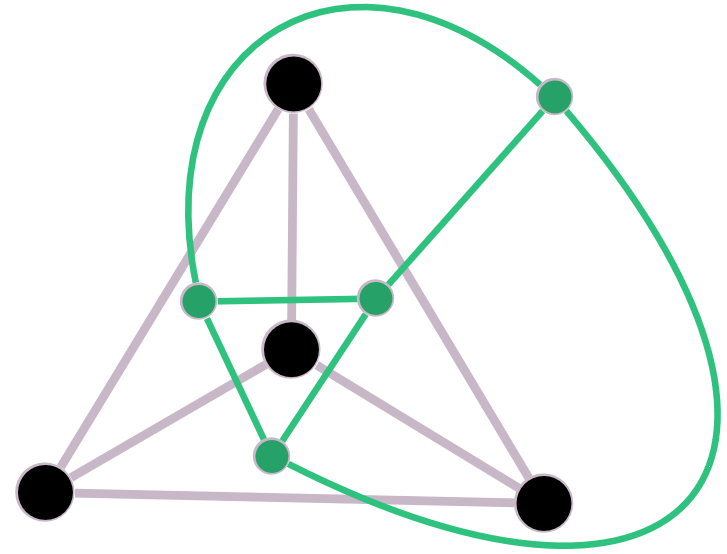
\includegraphics[width=4cm]{figures/duality/k4 with dual.png}
        \caption{A planar graph with its dual colored in green}
        \label{subfigure:k4-with-dual}
    \end{subfigure}\hfill%
    \begin{subfigure}{.3\textwidth}
        \centering
        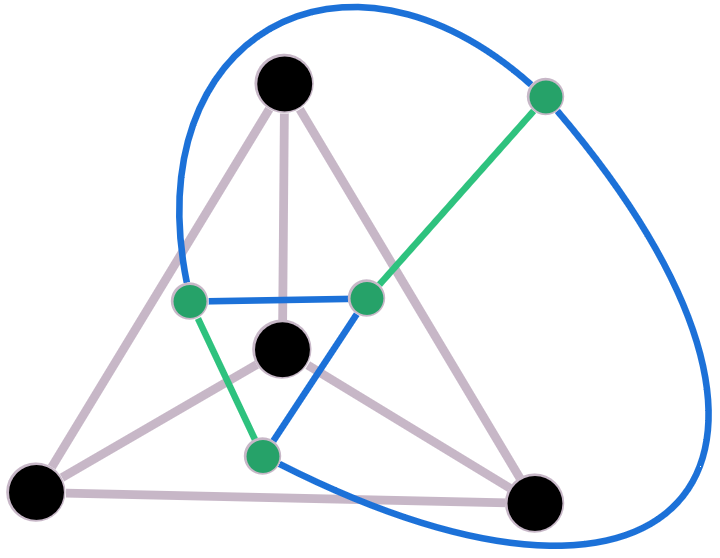
\includegraphics[width=4cm]{figures/duality/dual with cycle.png}
        \caption{A simple cycle in the dual, colored in blue}
        \label{figure:dual-with-cycle}
    \end{subfigure}\hfill%
    \begin{subfigure}{.3\textwidth}
        \centering
        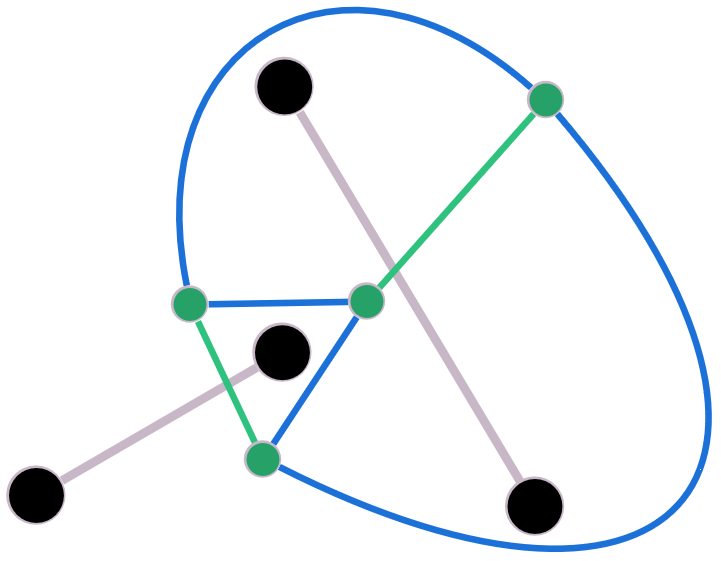
\includegraphics[width=4cm]{figures/duality/k4 cut in pieces.png}
        \caption{Deleting the edges that cross the dual's cycle cuts the graph in two}
        \label{subfigure:k4-cut}
    \end{subfigure}
    \caption{A simple cycle in a dual graph always corresponds to a cut in the original graph.}
    \label{figure:cycle-cut}
\end{figure}

\begin{theorem}[The relation between the number of vertices, edges and faces]
    Let $G~:= (V, E, \from, \too)$ be a connected planar graph, where $n~:= |V|, m~:= |E|$, and $f$ is the number of faces in any embedding of $G$. \\
    Claim: $n + f - m = 2$.

    \begin{proof}
        Let $H \sqsubseteq G$ be any non-empty connected subgraph that does not have any cycles, and let $n_H~:= |V(H)|$. Since it does not have any cycles, we have that:
        \begin{itemize}
            \item The outside face must be the only face: $f_H~:= 1$.
            \item Each edge must connect a 'new' vertex to the rest of the graph, except the first edge which connects two new vertices. Therefore the number of edges is one less than the number of vertices: $m_H~:= n_H - 1$.
        \end{itemize}
        We now have that $n_H + f_H - m_H = n_H + 1 - (n_H-1) = 2$, so the equality holds for this subgraph.

        Now we can iteratively add either an edge alone or both a vertex and an edge to $H$ until we have $G$. If we add just an edge, we increase both $m_H$ and $f_H$ by 1, and the equality still holds. If we add a new vertex with a new edge, we increase both $n_H$ and $m_h$ by one, and the equality still holds. 
        
        Therefore, the equality $n + f - m = 2$ holds for any connected planar graph $G$.
    \end{proof}
\end{theorem}

\begin{corollary}
    The number of faces is fixed. A graph may have different faces depending on the embedding, but the number of faces is always the same.
\end{corollary}
    
\begin{corollary}
    \label{corollary:m-leq-3n}
    Since all faces (except possibly the outer face) are bounded by at least three edges, and all edges touch at most two faces, we can show that if $n \geq 3$, then $m \leq 3n-6$.
\end{corollary}


\chapter{Shortest Odd Walk}
Before we start on the main topic of this thesis, we want to discuss a closely related problem:

\fbox{\parbox{0.94\textwidth}{\textsc{Shortest Odd Walk}\\
    \textbf{Input:} A weighted graph $G$, two vertices $s,t \in V$\\
    \textbf{Output:} the shortest $s$-$t$-walk in $G$ that uses an odd number of edges
}}

The difference is simple: a walk may use the same vertices multiple times, whereas a path can not. A naïve attempt at solving \textsc{Shortest Odd Path} will often accidentally use the same vertices multiple times, and then be an odd walk instead. Therefore, we want to present an algorithm to solve \textsc{Shortest Odd Walk} first, and explain why it does not solve \textsc{Shortest Odd Path}.

\section{Intuition}
Our algorithm will take inspiration from Dijkstra's algorithm for \textsc{Shortest Path}, and assume that all the edges have non-negative weights. Remember, in Dijkstra's algorithm we have an array to keep the tentative best distance to each vertex. In this algorithm, we will keep two such arrays, one for the best distance using an odd walk, and one for the best distance using an even walk. Each vertex can be scanned at most twice: once when we have found the definitive best odd walk and want to find potential improvements to the even walks of its neighbours, and similar when we find the best odd walk.


\section{Psuedocode}
Here is the psuedocode of the algorithm. To see the code implemented in Rust, see the GitHub repository \cite{source:codebase}.

\begin{lstlisting}[caption={Shortest Odd Walk},label=Listing,mathescape=true]
def shortest_odd_walk(graph, s, t) {
    for u in 0..n {
        even_dist[u] = $\infty$
        odd_dist[u] = $\infty$
        even_done[u] = false;
        odd_done[u] = false;
    }
    even_dist[s] = 0

    queue = priority_queue([(0, true, s)]);
    while queue is not empty {
        (dist_u, even, u) = queue.pop()
        if even {
            if even_done[u] continue;
            even_done[u] = true;

            for edge in graph[u] {
                v = to(edge);
                dist_v = dist_u + weight(edge);
                if dist_v < odd_dist[v] {
                    odd_dist[v] = dist_v;
                    queue.push((dist_v, false, v));
                }
            }
        }
        else {
            if odd_done[u] continue;
            odd_done[u] = true;

            for edge in graph[u] {
                v = to(edge);
                dist_v = dist_u + weight(edge);
                if dist_v < even_dist[v] {
                    even_dist[v] = dist_v;
                    queue.push((dist_v, true, v));
                }
            }
        }
        if odd_dist[t] < $\infty$ {
            return odd_dist[y];
        }
    }
    return None;
}
\end{lstlisting}

In the psuedocode we show how to find the best odd walk from the source vertex to the target vertex. If we instead want to find the best odd or even walks to all vertices, we can simply remove the if-clause around the target, and return the arrays instead.
\section{Analysis}

\begin{figure}
    \centering
    \begin{tikzpicture}
        \tikzstyle{every node}=[circle, fill=lightgray, draw=black, inner sep=2pt, minimum size=1.5em, font=\footnotesize, text=black]
        \tikzstyle{edge}=[gray, line width=1.5mm]
    
        \node (s) at (0,2) {$s$};
        \node (a) at (2,2) {$a$};
        \node (b) at (1,0) {$b$};
        \node (c) at (3,0) {$c$};
        \node (t) at (4,2) {$t$};
    
        \draw[edge] (s) -- (a) -- (b) -- (c) -- (a) -- (t);
    \end{tikzpicture}
    \caption{No odd $s$-$t$-path exist, yet we still have many odd $s$-$t$-walks.}
    \label{figure:small2}
 \end{figure}

Consider \Cref{figure:small2}. There are no odd paths from $s$ to $t$, yet we have an infinite amount of odd walks by utilizing the cycles $[a,b,c]$ or $[a,c,b]$ an odd number of times to offset the parity. Our algorithm would first find an odd walk to $a$, then an even walk to $b$, then an odd walk to $c$, then an even walk to $a$, and lastly an odd walk to $t$. However, then $a$ is used twice in the walk, once for each parity, and the resulting walk is not a path. Therefore can this algorithm not be used to solve \textsc{Shortest Odd Path}.

\subsection{Limitations}
The main limitation of the algorithm is that the edges in the input graph must have either non-negative weights or no weights at all. Otherwise we cannot guarantee that \pyth{even_dist[u]} and \pyth{odd_dist[u]} have their final, correct values when we scan a vertex $u$. 

Note that unlike most other algorithms shown in this thesis, this algorithm does not require the input graph to be undirected, it can also be directed.

\subsection{Correctness}
Let \pyth{(priority, even, u)} be the triple at the front of the queue at any point in the execution of our algorithm.
Claim: If \pyth{even} is true and \pyth{even_done[u]} is false, then \pyth{priority} is the cost of the shortest even path from the source to \pyth{u}.

\begin{proof}
By induction. 

The source vertex \pyth{s} has a best possible even cost of \pyth{0}, and initially we have only \pyth{(0, true, s)} in the queue. When that triple is popped the property holds in the base case.

\todo[inline]{
    Burde yoinke beviset herfra: https://web.engr.oregonstate.edu/~glencora/wiki/uploads/dijkstra-proof.pdf

    Eller herfra: https://community.wvu.edu/~krsubramani/courses/fa05/gaoa/qen/dijk.pdf

    Eller fra INF234

    Også si det samme når det er odd, kanskje
}

\end{proof}

\subsection{Complexity}
Let $(G,s,t)$ be an instance of \textsc{Shortest Odd Walk}, let $n := |V|$ and let $m := |E|$.\\
Claim: the algorithm runs in time at most $O(m \cdot \log m)$, or $O(m \cdot \log n)$ if the graph is simple.
\begin{proof}
    Because of our \pyth{odd_done} and \pyth{even_done} arrays, we can guarantee that each vertex is scanned at most twice, once for each parity. For each scan, we loop through each of the neighbours in linear time, and consider putting them in the queue. The total cost of the scans is therefore at most $O(m)$. A vertex may be put into the queue many times before it is scanned, in the worst case once for each of its neighbours. That means that we put vertices in the queue at most $O(m)$ times, for a total cost of $O(m)$, and removing all of them takes a total of $O(m \cdot \log m)$. 
    
    The algorithm runs in time at most $O(m) + O(m \cdot \log m) = O(m \cdot \log m)$, which shows the first part of the claim.
    
    If the graph is simple we may simplify the complexity further: $O(m \cdot \log m) \subseteq (m \cdot \log n^2) = O(m \cdot 2 \cdot \log n) = O(m \cdot \log n)$, which shows the second part of the claim.
\end{proof}

\subsection{Benchmarking}

\todo[inline]{Do the benchmarking, silly}

\subsection{Discussion}
Though we discovered it ourselves, the algorithm is not particularly groundbreaking or in any way creative. Thus, we do not expect it to be original. It is, however, quite fast, and we are happy with that. The main reason we include it in this thesis is because of its pedagogical value in introducing our main topic: \textsc{Shortest Odd Path}. \todo{Skrive mer her?}

\chapter{Shortest Odd Path}
Now that we have tried out some algorithms for \textsc{Shortest Odd Walk}, we are finally ready to add the restriction that each vertex is used at most once, and thus solve \textsc{Shortest Odd Path}. The algorithm we are about to present is based on Derigs' algorithm \cite{source:derigs_shortest_odd_path}, \todo{Improvements? Simplifications? Modifications? Improved presentation?}though with some improvements.

\section{Reduction to \textsc{Shortest Alternating Path}}
\label{subsection:reduction}
Consider first another related problem:

\noindent\fbox{\parbox{0.94\textwidth}{\textsc{Shortest Alternating Path}\\
    \textbf{Input:} a weighted graph $G := (V, E, \from, \too, \weight)$, two vertices $s,t \in V$, and a set $F \subseteq E$\\
    \textbf{Output:} an $s$-$t$-path in $G$ of minimum cost, where every other edge used is in $F$.
}}

Derigs observed that \textsc{Shortest Odd Path} can be reduced to a special case of \textsc{Shortest Alternating Path}, by constructing what we will refer to as a $\emph{mirror graph}$. \todo{Dobbelsjekk dette, men \textsc{Shortest Alternating Path} er antagelig NP-komplett og vi burde nevne det før vi sier at vi skal løse et spesialtilfelle.}

\begin{definition}[Mirror graph]
    \label{def:mirror-graph}
    Let $G = (V, E)$ be a graph, and $s,t \in V$ be two vertices.
    We construct a new graph $H \sqsupset G$, where for each vertex $u \in V \setminus \{s,t\}$ we add a 'mirror' vertex $u'$, and a connecting 'mirror' edge between them. 
    The vertices in $V(H)$ that are also in $V(G)$ are referred to as the 'real' vertices, and the newly added vertices are referred to as the 'mirror' vertices. In addition, for any vertex $u \in V(H) \setminus \{s,t\}$, real or not, we define $\mirror(u)$ as $u$'s mirror on the other side. We usually label mirror vertices with an $'$ at the end of the real counterpart's label.
    For example, if $G$ is the graph in \Cref{figure:input-graph}, then \Cref{figure:mirror-graph} would be its corresponding mirror graph $H$.
\end{definition}
\todo[inline]{We have to standardize what we call the different edges in a mirror graph. And also actually add the edges to the mirror graph at all in the definition.}

\begin{figure}[H]
    \centering
    \begin{subfigure}{.45\textwidth}
        \begin{tikzpicture}
            \tikzstyle{every node}=[circle, fill=lightgray, draw=black, inner sep=2pt, minimum size=1.5em, font=\footnotesize, text=black]
            \tikzstyle{edge}=[gray, line width=1.5mm]
       
            \node (s) at (0.5,1) {$s$};
            \node (a) at (2,2) {$a$};
            \node (b) at (3,0.6) {$b$};
            \node (c) at (4,2) {$c$};
            \node (d) at (5.5,1) {$d$};
            \node (t) at (7,1.5) {$t$};
       
            \draw[edge] (s) -- (a) -- (c) -- (d) -- (t);
            \draw[edge] (a) -- (b) -- (c);
          \end{tikzpicture}
          \caption{The input graph $G$}
          \label{figure:input-graph}
    \end{subfigure}\hfill%
    \begin{subfigure}{.45\textwidth}
        \begin{tikzpicture}
            \tikzstyle{every node}=[circle, fill=lightgray, draw=black, inner sep=2pt, minimum size=1.5em, font=\footnotesize, text=black]
            \tikzstyle{edge}=[gray, line width=1.5mm]
       
            \node (s) at (0.5,1) {$s$};
            \node (a) at (2,2) {$a$};
            \node (b) at (3,0.6) {$b$};
            \node (c) at (4,2) {$c$};
            \node (d) at (5.5,1) {$d$};
            \node (t) at (7,1.5) {$t$};

            \node (a') at (2,4) {$a'$};
            \node (b') at (3,2.6) {$b'$};
            \node (c') at (4,4) {$c'$};
            \node (d') at (5.5,3) {$d'$};
       
            \draw[edge] (s) -- (a) -- (c) -- (d) -- (t);
            \draw[edge] (a) -- (b) -- (c);

            \draw[edge] (a') -- (b') -- (c') -- (d');
            \draw[edge] (a') -- (c');

            \tikzstyle{edge}=[red, line width=1.5mm]
            \draw[edge] (a) -- (a');
            \draw[edge] (b) -- (b');
            \draw[edge] (c) -- (c');
            \draw[edge] (d) -- (d');
        \end{tikzpicture}
        \caption{The mirror graph $H$ of $G$, mirror edges marked in red}
        \label{figure:mirror-graph}
    \end{subfigure}
    \caption{Reduction from \textsc{Shortest Odd Path} to \textsc{Shortest Alternating Path}.}
 \end{figure}

Our reduction from \textsc{Shortest Odd Path} to \textsc{Shortest Alternating Path} follows:
\begin{enumerate}
    \item Let $(G, s, t)$ be an instance of \textsc{Shortest Odd Path}.
    \item Construct $H$ as the mirror graph of $G$, and let $F$ be the set of mirror edges in $H$. Now $(H, s, t, F)$ is an instance of \textsc{Shortest Alternating Path}.
    \item Let $P'$ be the shortest alternating path of $(H, s, t, F)$, if one exists. If none exist, then we do not have any odd $s$-$t$-paths in $G$ either.
    \item Construct $P$ by filtering out mirror edges from $P'$, and for each edge $(u',v') \in E(H) \setminus (F \cup E(G))$ from the mirror side of $H$ we replace it by the corresponding edge $(u,v) \in E(G)$ from the real side.
    \label{point:translate_alternating_path}
    \item Now $P$ is the shortest odd $s$-$t$-path in $G$.
\end{enumerate}

For example, if our input $G$ for \textsc{Shortest Odd Path} is \Cref{figure:input-graph}, then $H$ and $F$ could look like \Cref{figure:mirror-graph}. One of the two possible alternating paths is $P' := [(s,a), (a, a'), (a',b'), (b',b)$, $(b,c), (c,c'), (c',d'), (d',d), (d,t)]$. When we filter out mirror edges and replace edges from the mirror side with their real counterparts, we end up with $P := [(s,a),(a,b),(b,c),(c,d),(d,t)]$, which is the shortest odd $s$-$t$-path in $G$. 
\todo{dette kan kanskje formuleres bedre?}

Now that we have two copies of most vertices in $H$, we run the risk of accidentally using the same vertex multiple times and ending up with a walk rather than a path in $G$. The key is that $F$ is an (almost) perfect matching, and when we step on a vertex $u$ we have to take the mirror edge and step on $\mirror(u)$ next. So both copies have to be used directly after each other, and when we filter out the mirror edges the copies are effectively merged to just a single step in the path. Therefore, vertices are never repeated and we end up with a path.

To see why the reduction necessarily yields an \emph{odd} path, simply observe that for each step we take in the graph, we have to go to the other side of the mirror. If we take another step, we get back to the same side again. It is only when we reach the target vertex $t$ that we do not have to go to the other side. Therefore, to reach a neighbour of $t$, we must have used an even number of mirror edges and an even number of non-mirror edges, and when we take the last step to reach $t$ we have used an odd number of edges and thus found an odd path. If this alternating $s$-$t$-path in $H$ is the shortest such path, then the corresponding path in $G$ must also be the shortest odd $s$-$t$-path in $G$. 

\todo{May not have to write this, if we define mirror graphs better}
The reduction works also in the weighted case, as long as each edge on the mirror side get the same weight as their real counterpart, and all the mirror edges get the same (usually 0) weight. The interested reader may see \cite{source:derigs_shortest_odd_path} for more details on this reduction.

Ball and Derigs \cite{source:shortest_alternating_path} have shown how to efficiently solve \textsc{Shortest Alternating Path}. In their algorithms, subgraphs are shrunk into pseudonodes whenever possible, to make the graph smaller. The drawback is that certain pseudonodes must later be expanded again, which is the most complicated and expensive part of their algorithms. In our case, however, we have a special case of \textsc{Shortest Alternating Path}. The set $F$ is, with the exception of $s$ and $t$, a perfect matching of $H$, and we will therefore never have to expand pseudonodes after shrinking them. The curious reader may visit \cite{source:shortest_alternating_path} for more on these algorithms and why our almost-perfect matching is a simpler case.

\section{The idea for our \textsc{Shortest Alternating Path} algorithm}
We will explain the general idea of our algorithm by following an example, and solve for the graph in \Cref{figure:input-graph}. First we construct the mirror graph like explained in \Cref{subsection:reduction}, to produce the graph in \Cref{figure:mirror-graph}. Then we initialize an empty priority queue of vertices and edges to be scanned. For each vertex $u \in V(H)$, we denote
\begin{itemize}
    \item $d^+_u :=$ the length of the shortest alternating $s$-$u$-path ending on a mirror edge
    \item $d^-_u :=$ the length of the shortest alternating $s$-$u$-path ending on a non-mirror edge
    \item $\pred_u :=$ the last edge used to find $u$'s most recent value for $d^-_u$
\end{itemize}

Initally these are either $\infty$ or undefined, except for the source vertex $s$, where we can set $d^+_s := 0$. Then, for each edge $e \in N(s)$, we can set $d^-_{\too(e)} := \weight(e)$, $pred_{to(e)} := e$, and add $\too(e)$ to our priority queue with priority $2 \cdot \weight(e)$.

We visualize it in the diagram below.

\begin{minipage}{.75\linewidth}
    \begin{tikzpicture}{text centered}
        \tikzstyle{every node}=[rectangle, fill=lightgray, draw=black, inner sep=2pt, minimum size=1.5em, font=\footnotesize, text=black]
        \tikzstyle{edge}=[gray, line width=1mm]
   
        \node (s) at (0,1)    {\begin{tabular}{c} $s$  \\ $d^+:0$       \\ $d^-:\infty$ \end{tabular}};
        \node (a) at (2,2)    {\begin{tabular}{c} $a$  \\ $d^+:\infty$  \\ $d^-:1$      \end{tabular}};
        \node (b) at (4,0)    {\begin{tabular}{c} $b$  \\ $d^+:\infty$  \\ $d^-:\infty$ \end{tabular}};
        \node (c) at (6,2)    {\begin{tabular}{c} $c$  \\ $d^+:\infty$  \\ $d^-:\infty$ \end{tabular}};
        \node (d) at (8,0)    {\begin{tabular}{c} $d$  \\ $d^+:\infty$  \\ $d^-:\infty$ \end{tabular}};
        \node (t) at (10,1)   {\begin{tabular}{c} $t$  \\ $d^+:\infty$  \\ $d^-:\infty$ \end{tabular}};

        \node (a') at (2,5)   {\begin{tabular}{c} $a'$ \\ $d^+:\infty$  \\ $d^-:\infty$ \end{tabular}};
        \node (b') at (4,3.5) {\begin{tabular}{c} $b'$ \\ $d^+:\infty$  \\ $d^-:\infty$ \end{tabular}};
        \node (c') at (6,5)   {\begin{tabular}{c} $c'$ \\ $d^+:\infty$  \\ $d^-:\infty$ \end{tabular}};
        \node (d') at (8,3)   {\begin{tabular}{c} $d'$ \\ $d^+:\infty$  \\ $d^-:\infty$ \end{tabular}};
   
        \draw[edge] (s) -- (a) -- (c) -- (d) -- (t);
        \draw[edge] (a) -- (b) -- (c);

        \draw[edge] (a') -- (b') -- (c') -- (d');
        \draw[edge] (a') -- (c');

        \tikzstyle{edge}=[red, line width=1.5mm]
        \draw[edge] (a) -- (a');
        \draw[edge] (b) -- (b');
        \draw[edge] (c) -- (c');
        \draw[edge] (d) -- (d');
    \end{tikzpicture}
\end{minipage}\hfill%
\begin{minipage}{.22\linewidth}
    Queue:
    \begin{itemize}
        \item Vertex(2,$a$)
    \end{itemize}
\end{minipage}

The first and only vertex in the queue is $a$. We pop it, set $d^+_{a'} := d^-_a$, and 'scan'~$a'$. By that, we mean to look at each neighbour $e \in G[a']$, and see if our new value $d^+_{a'} + \weight(e)$ is better than the previous value $d^-_{\too(edge)}$. That is the case for both~$b'$ and~$c'$, so we update their values and add them to the queue. Their priorities in the queue is equal to twice their $d^-$ values, which is $2 \cdot 2 = 4$ for both of them.

\begin{minipage}{.75\linewidth}
    \begin{tikzpicture}{text centered}
        \tikzstyle{every node}=[rectangle, fill=lightgray, draw=black, inner sep=2pt, minimum size=1.5em, font=\footnotesize, text=black]
        \tikzstyle{edge}=[gray, line width=1mm]
   
        \node (s) at (0,1)    {\begin{tabular}{c} $s$  \\ $d^+:0$       \\ $d^-:\infty$ \end{tabular}};
        \node (a) at (2,2)    {\begin{tabular}{c} $a$  \\ $d^+:\infty$  \\ $d^-:1$      \end{tabular}};
        \node (b) at (4,0)    {\begin{tabular}{c} $b$  \\ $d^+:\infty$  \\ $d^-:\infty$ \end{tabular}};
        \node (c) at (6,2)    {\begin{tabular}{c} $c$  \\ $d^+:\infty$  \\ $d^-:\infty$ \end{tabular}};
        \node (d) at (8,0)    {\begin{tabular}{c} $d$  \\ $d^+:\infty$  \\ $d^-:\infty$ \end{tabular}};
        \node (t) at (10,1)   {\begin{tabular}{c} $t$  \\ $d^+:\infty$  \\ $d^-:\infty$ \end{tabular}};

        \node (a') at (2,5)   {\begin{tabular}{c} $a'$ \\ $d^+:1$       \\ $d^-:\infty$ \end{tabular}};
        \node (b') at (4,3.5) {\begin{tabular}{c} $b'$ \\ $d^+:\infty$  \\ $d^-:2$      \end{tabular}};
        \node (c') at (6,5)   {\begin{tabular}{c} $c'$ \\ $d^+:\infty$  \\ $d^-:2$      \end{tabular}};
        \node (d') at (8,3)   {\begin{tabular}{c} $d'$ \\ $d^+:\infty$  \\ $d^-:\infty$ \end{tabular}};
   
        \draw[edge] (s) -- (a) -- (c) -- (d) -- (t);
        \draw[edge] (a) -- (b) -- (c);

        \draw[edge] (a') -- (b') -- (c') -- (d');
        \draw[edge] (a') -- (c');

        \tikzstyle{edge}=[red, line width=1.5mm]
        \draw[edge] (a) -- (a');
        \draw[edge] (b) -- (b');
        \draw[edge] (c) -- (c');
        \draw[edge] (d) -- (d');
    \end{tikzpicture}
\end{minipage}\hfill%
\begin{minipage}{.26\linewidth}
    Queue:
    \begin{itemize}
        \item \st{Vertex(2,$a$)}
        \item Vertex(4,$b'$)
        \item Vertex(4,$c'$)
    \end{itemize}
\end{minipage}

The next vertex in the queue is $b'$, so we set $d^+_b := d^-_{b'}$ and scan $b'$:

\begin{minipage}{.75\linewidth}
    \begin{tikzpicture}{text centered}
        \tikzstyle{every node}=[rectangle, fill=lightgray, draw=black, inner sep=2pt, minimum size=1.5em, font=\footnotesize, text=black]
        \tikzstyle{edge}=[gray, line width=1mm]
   
        \node (s) at (0,1)    {\begin{tabular}{c} $s$  \\ $d^+:0$       \\ $d^-:\infty$ \end{tabular}};
        \node (a) at (2,2)    {\begin{tabular}{c} $a$  \\ $d^+:\infty$  \\ $d^-:1$      \end{tabular}};
        \node (b) at (4,0)    {\begin{tabular}{c} $b$  \\ $d^+:2$       \\ $d^-:\infty$ \end{tabular}};
        \node (c) at (6,2)    {\begin{tabular}{c} $c$  \\ $d^+:\infty$  \\ $d^-:3     $ \end{tabular}};
        \node (d) at (8,0)    {\begin{tabular}{c} $d$  \\ $d^+:\infty$  \\ $d^-:\infty$ \end{tabular}};
        \node (t) at (10,1)   {\begin{tabular}{c} $t$  \\ $d^+:\infty$  \\ $d^-:\infty$ \end{tabular}};

        \node (a') at (2,5)   {\begin{tabular}{c} $a'$ \\ $d^+:1$       \\ $d^-:\infty$ \end{tabular}};
        \node (b') at (4,3.5) {\begin{tabular}{c} $b'$ \\ $d^+:\infty$  \\ $d^-:2$      \end{tabular}};
        \node (c') at (6,5)   {\begin{tabular}{c} $c'$ \\ $d^+:\infty$  \\ $d^-:2$      \end{tabular}};
        \node (d') at (8,3)   {\begin{tabular}{c} $d'$ \\ $d^+:\infty$  \\ $d^-:\infty$ \end{tabular}};
   
        \draw[edge] (s) -- (a) -- (c) -- (d) -- (t);
        \draw[edge] (a) -- (b) -- (c);

        \draw[edge] (a') -- (b') -- (c') -- (d');
        \draw[edge] (a') -- (c');

        \tikzstyle{edge}=[red, line width=1.5mm]
        \draw[edge] (a) -- (a');
        \draw[edge] (b) -- (b');
        \draw[edge] (c) -- (c');
        \draw[edge] (d) -- (d');
    \end{tikzpicture}
\end{minipage}\hfill%
\begin{minipage}{.26\linewidth}
    Queue:
    \begin{itemize}
        \item \st{Vertex(4,$b'$)}
        \item Vertex(4,$c'$)
        \item Vertex(6,$c$)
    \end{itemize}
\end{minipage}

Now $c'$ is the next in the queue, we set $d^+_c := d^-c'$ and scan $c'$. This is where the interesting part happens: now we have set both $d^+$ and $d^-$ for $b$ and $c$, and that means that we have found an odd cycle in the graph. The edge between them, $e$, is called the \emph{blossom edge}, and is marked in green. We add $e$ to the queue, with the priority $d^+_c + d^+_b + \weight(e)$.

\begin{minipage}{.75\linewidth}
    \begin{tikzpicture}{text centered}
        \tikzstyle{every node}=[rectangle, fill=lightgray, draw=black, inner sep=2pt, minimum size=1.5em, font=\footnotesize, text=black]
        \tikzstyle{edge}=[gray, line width=1mm]
   
        \node (s) at (0,1)    {\begin{tabular}{c} $s$  \\ $d^+:0$       \\ $d^-:\infty$ \end{tabular}};
        \node (a) at (2,2)    {\begin{tabular}{c} $a$  \\ $d^+:\infty$  \\ $d^-:1$      \end{tabular}};
        \node (b) at (4,0)    {\begin{tabular}{c} $b$  \\ $d^+:2$       \\ $d^-:3$      \end{tabular}};
        \node (c) at (6,2)    {\begin{tabular}{c} $c$  \\ $d^+:2$       \\ $d^-:3$      \end{tabular}};
        \node (d) at (8,0)    {\begin{tabular}{c} $d$  \\ $d^+:\infty$  \\ $d^-:4$      \end{tabular}};
        \node (t) at (10,1)   {\begin{tabular}{c} $t$  \\ $d^+:\infty$  \\ $d^-:\infty$ \end{tabular}};

        \node (a') at (2,5)   {\begin{tabular}{c} $a'$ \\ $d^+:1$       \\ $d^-:\infty$ \end{tabular}};
        \node (b') at (4,3.5) {\begin{tabular}{c} $b'$ \\ $d^+:\infty$  \\ $d^-:2$      \end{tabular}};
        \node (c') at (6,5)   {\begin{tabular}{c} $c'$ \\ $d^+:\infty$  \\ $d^-:2$      \end{tabular}};
        \node (d') at (8,3)   {\begin{tabular}{c} $d'$ \\ $d^+:\infty$  \\ $d^-:\infty$ \end{tabular}};
   
        \draw[edge] (s) -- (a) -- (c) -- (d) -- (t);
        \draw[edge] (a) -- (b);

        \draw[edge] (a') -- (b') -- (c') -- (d');
        \draw[edge] (a') -- (c');

        \tikzstyle{edge}=[red, line width=1.5mm]
        \draw[edge] (a) -- (a');
        \draw[edge] (b) -- (b');
        \draw[edge] (c) -- (c');
        \draw[edge] (d) -- (d');

        \tikzstyle{edge}=[green, line width=1mm]
        \draw[edge] (b) -- (c);
    \end{tikzpicture}
\end{minipage}\hfill%
\begin{minipage}{.26\linewidth}
    Queue:
    \begin{itemize}
        \item \st{Vertex(4,$c'$)}
        \item Blossom(5,($b$,$c$))
        \item Vertex(6,$c$)
        \item Vertex(6,$d$)
    \end{itemize}
\end{minipage}

Next up is to scan this blossom edge, and compute its corresponding odd cycle by backtracking from $c$ and $b$ until they meet at $a'$. To visualize the cycle, we like to 'stretch out' the graph a little, and draw it like below. Note that some of the edges are omitted for clarity. Now we can see that the cycle consists of [$a',c',c,b,b',a'$]. We call the set $\mathbb{B} := \{c',c,b,b'\}$ a \emph{blossom}, and $a'$ the \emph{base} of the blossom, inspired by the famous Blossom algorithm by \cite{source:blossom}.

\begin{minipage}{.7\linewidth}
    \begin{tikzpicture}{text centered}
        \tikzstyle{every node}=[rectangle, fill=lightgray, draw=black, inner sep=2pt, minimum size=1.5em, font=\footnotesize, text=black]
        \tikzstyle{edge}=[gray, line width=1mm]
   
        \node (s) at (0,1)    {\begin{tabular}{c} $s$  \\ $d^+:0$       \\ $d^-:\infty$ \end{tabular}};
        \node (a) at (2,1)    {\begin{tabular}{c} $a$  \\ $d^+:\infty$  \\ $d^-:1$      \end{tabular}};
        \node (b) at (8,0)    {\begin{tabular}{c} $b$  \\ $d^+:2$       \\ $d^-:3$      \end{tabular}};
        \node (c) at (8,2)    {\begin{tabular}{c} $c$  \\ $d^+:2$       \\ $d^-:3$      \end{tabular}};
        \node (d) at (9,4)    {\begin{tabular}{c} $d$  \\ $d^+:\infty$  \\ $d^-:4$      \end{tabular}};
        \node (t) at (11,4)   {\begin{tabular}{c} $t$  \\ $d^+:\infty$  \\ $d^-:\infty$ \end{tabular}};

        \node (a') at (4,1)   {\begin{tabular}{c} $a'$ \\ $d^+:1$       \\ $d^-:\infty$ \end{tabular}};
        \node (b') at (6,0)   {\begin{tabular}{c} $b'$ \\ $d^+:\infty$  \\ $d^-:2$      \end{tabular}};
        \node (c') at (6,2)   {\begin{tabular}{c} $c'$ \\ $d^+:\infty$  \\ $d^-:2$      \end{tabular}};
        \node (d') at (7,4)   {\begin{tabular}{c} $d'$ \\ $d^+:\infty$  \\ $d^-:\infty$ \end{tabular}};
   
        \draw[edge] (s) -- (a) -- (a') -- (c') -- (d');
        \draw[edge] (a') -- (b');
        \draw[edge] (c) -- (d) -- (t);

        \tikzstyle{edge}=[red, line width=1.5mm]
        \draw[edge] (a) -- (a');
        \draw[edge] (b) -- (b');
        \draw[edge] (c) -- (c');
        \draw[edge] (d) -- (d');

        \tikzstyle{edge}=[green, line width=1.5mm]
        \draw[edge] (b) -- (c);
    \end{tikzpicture}
\end{minipage}\hfill%
\begin{minipage}{.26\linewidth}
    \vspace{2cm}
    Queue:
    \begin{itemize}
        \item Blossom(5,($b$,$c$))
        \item Vertex(6,$c$)
        \item Vertex(6,$d$)
    \end{itemize}
\end{minipage}

The first reason why we care about this blossom is because now we can immediately set the final, optimal $d^-$ and $d^+$ for all the vertices in the blossom. That is because we now have two alternating paths to each vertex, one goes around the cycle while the other takes the shortcut. One of these ends up on a mirror edge, and the other on a normal edge. For example, to go from $s$ to $c'$, we can either go through [$s,a,a',c'$] with a cost of $d^-_c$, or go along [$s,a,a',b',b,c,c'$] with a cost of $d^+_c$.

More specifically, for each $u \in \mathbb{B}$: \begin{itemize}
    \item If $d^+_u = \infty$, we set $d^+_u = d^-_{\mirror(u)}$.
    \item If we can improve $d^-_u$ by coming from its neighbour in the blossom, we do so.
\end{itemize}
After all these values have been set, we immediately scan all the vertices in $\mathbb{B}$ that just received values for $d^+$. In this example we scan $c'$ and $b'$, and discover $d'$. Unfortunately, since this is a very small blossom we don't have any vertices that receive new values for $d^-$.

\begin{minipage}{.7\linewidth}
    \begin{tikzpicture}{text centered}
        \tikzstyle{every node}=[rectangle, fill=lightgray, draw=black, inner sep=2pt, minimum size=1.5em, font=\footnotesize, text=black]
        \tikzstyle{edge}=[gray, line width=1mm]
   
        \node (s) at (0,1)    {\begin{tabular}{c} $s$  \\ $d^+:0$       \\ $d^-:\infty$ \end{tabular}};
        \node (a) at (2,1)    {\begin{tabular}{c} $a$  \\ $d^+:\infty$  \\ $d^-:1$      \end{tabular}};
        \node (b) at (8,0)    {\begin{tabular}{c} $b$  \\ $d^+:2$       \\ $d^-:3$      \end{tabular}};
        \node (c) at (8,2)    {\begin{tabular}{c} $c$  \\ $d^+:2$       \\ $d^-:3$      \end{tabular}};
        \node (d) at (9,4)    {\begin{tabular}{c} $d$  \\ $d^+:\infty$  \\ $d^-:4$      \end{tabular}};
        \node (t) at (11,4)   {\begin{tabular}{c} $t$  \\ $d^+:\infty$  \\ $d^-:\infty$ \end{tabular}};

        \node (a') at (4,1)   {\begin{tabular}{c} $a'$ \\ $d^+:1$       \\ $d^-:\infty$ \end{tabular}};
        \node (b') at (6,0)   {\begin{tabular}{c} $b'$ \\ $d^+:3$       \\ $d^-:2$      \end{tabular}};
        \node (c') at (6,2)   {\begin{tabular}{c} $c'$ \\ $d^+:3$       \\ $d^-:2$      \end{tabular}};
        \node (d') at (7,4)   {\begin{tabular}{c} $d'$ \\ $d^+:\infty$  \\ $d^-:4$      \end{tabular}};
   
        \draw[edge] (s) -- (a) -- (a') -- (c') -- (d');
        \draw[edge] (a') -- (b');
        \draw[edge] (c) -- (d) -- (t);

        \tikzstyle{edge}=[red, line width=1.5mm]
        \draw[edge] (a) -- (a');
        \draw[edge] (b) -- (b');
        \draw[edge] (c) -- (c');
        \draw[edge] (d) -- (d');

        \tikzstyle{edge}=[green, line width=1.5mm]
        \draw[edge] (b) -- (c);
    \end{tikzpicture}
\end{minipage}\hfill%
\begin{minipage}{.26\linewidth}
    \vspace{2cm}
    Queue:
    \begin{itemize}
        \item \st{Blossom(5,($b$,$c$))}
        \item Vertex(6,$c$)
        \item Vertex(6,$d$)
        \item Vertex(8,$d'$)
    \end{itemize}
\end{minipage}

The second reason we compute the blossom is that we no longer care much about the individual vertices in $\mathbb{B}$, and can shrink it into just the base $a'$. We will still scan vertices like $c$ from the queue as before, but whenever we are backtracking to compute blossoms we can skip the verties in $\mathbb{B}$ entirely and go straight to the base $a'$ instead. In this example, in a few iterations the algorithm will find either $(d',a')$ or $(d,a')$ as a blossom edge, with just $\{d,d'\}$ as its blossom and $a'$ as the base here as well. If we didn't contract the previous blossom, this new blossom would instead consist of $\{c',c,b,b',d,d'\}$, but we are already completely done with most of those vertices and computing all of it again would be a waste. Therefore we shrink them. 

If the reader is familiar with the more general \textsc{Shortest Alternating Path} algorithm \cite{source:shortest_alternating_path} or the original blossom algorithm \cite{source:blossom}, and worry that such pseudonodes often have to be expanded again, then remember that in our case the set $F$ is an almost-perfect matching and those cases never happen. \todo{trenger vi si dette? Droppe det? Formulere det annerledes?}

\begin{minipage}{.7\linewidth}
    \begin{tikzpicture}{text centered}
        \tikzstyle{every node}=[rectangle, fill=lightgray, draw=black, inner sep=2pt, minimum size=1.5em, font=\footnotesize, text=black]
        \tikzstyle{edge}=[gray, line width=1mm]
   
        \node (s)  at (0,1) {\begin{tabular}{c} $s$  \\ $d^+:0$       \\ $d^-:\infty$ \end{tabular}};
        \node (a)  at (2,1) {\begin{tabular}{c} $a$  \\ $d^+:\infty$  \\ $d^-:1$      \end{tabular}};
        \node (a') at (4,1) {\begin{tabular}{c} $a'$ \\ $d^+:1$       \\ $d^-:\infty$ \end{tabular}};
        \node (d)  at (6,2) {\begin{tabular}{c} $d$  \\ $d^+:\infty$  \\ $d^-:4$      \end{tabular}};
        \node (d') at (6,0) {\begin{tabular}{c} $d'$ \\ $d^+:\infty$  \\ $d^-:4$      \end{tabular}};
        \node (t)  at (8,2) {\begin{tabular}{c} $t$  \\ $d^+:\infty$  \\ $d^-:\infty$ \end{tabular}};
        
        \draw[edge] (s) -- (a);
        \draw[edge] (a') -- (d) -- (t);
        \draw[edge] (a') -- (d');

        \tikzstyle{edge}=[red, line width=1.5mm]
        \draw[edge] (a) -- (a');
        \draw[edge] (d) -- (d');
    \end{tikzpicture}
\end{minipage}\hfill%
\begin{minipage}{.26\linewidth}
    \vspace{2cm}
    Queue:
    \begin{itemize}
        \item Vertex(6,$c$)
        \item Vertex(6,$d$)
        \item Vertex(8,$d'$)
    \end{itemize}
\end{minipage}

Let us now skip a few steps, until $t$ eventually reaches the front of the queue. At that point we have that $d^-_t = 5$, and that is also the cost of the shortest odd path in our original input graph. To compute the exact path we can backtrack from $t$ to $s$ and then translate that path as described in Step \ref{point:translate_alternating_path} of our reduction in \Cref{subsection:reduction}. We end up with the path [$(s,a),(a,b),(b,c),(c,d),(d,t)$], which is the shortest odd $s$-$t$-path in the graph.

\section{Psuedocode}

\subsection{Initialization and the main control loop}
\begin{lstlisting}[caption={Main},label=Listing,mathescape=true]
fn main(input_graph, s, t){
    init(input_graph, s, t);

    while ! control() {}

    if d_minus[t] == $\infty$ {
        // The graph is a no-instance, no odd s-t-paths exist
        return None;
    }

    current_edge = pred[t];
    path = [current_edge];
    while from(current_edge) != s {
        current_edge = pred[mirror(from(current_edge))];
        if from(current_edge) < input_graph.n() {
            path.push(current_edge);
        }
        else {
            path.push(shift_edge_by(current_edge, -input_graph.n()));
        }
    }
    return Some(d_minus[t], path);
}
\end{lstlisting}

\begin{lstlisting}[caption={Initialization},label=Listing,mathescape=true]
fn init(input_graph, s, t) {
    graph = create_mirror_graph(input_graph);

    for u in 0..n {
        d_plus[u] = $\infty$;
        d_minus[u] = $\infty$;
        pred[u] = null;
        completed[u] = false;
        basis[u] = u;
    }
    d_plus[s] = 0;
    completed[s] = true;

    for edge in graph[s] {
        pq.push(Vertex(weight(edge), to(edge)));
        d_minus[to(edge)] = weight(edge);
        pred[to(edge)] = e;
    }
}
\end{lstlisting}

\begin{lstlisting}[caption={Control, the main loop},label=Listing,mathescape=true]
fn control() -> bool {
    while ! pq.is_empty() {
        match pq.top() {
            Vertex(_, u) => {
                if completed[u] {
                    pq.pop();
                }
                else {
                    break;
                }
            },
            Blossom(_, edge) => {
                if base_of(from(edge)) == base_of(to(edge)) {
                    pq.pop();
                }
                else {
                    break;
                }
            }
        }
    }

    if pq.is_empty() {
        // No odd s-t-paths in G exist :(
        return true;
    }
    match pq.pop() {
        Vertex(delta, l) => {
            if l == t {
                // We have found a shortest odd s-t-path has been found :)
                return true;
            }
            grow(l);
        }
        Blossom(delta, edge) => {
            blossom(e);
        }
    }
    return false;
}
\end{lstlisting}

\subsection{Scanning vertices}
\begin{lstlisting}[caption={Grow},label=Listing,mathescape=true]
fn grow(l) {
    d_plus[mirror(l)] = d_minus[l];
    scan(mirror(l));
}
\end{lstlisting}

\begin{lstlisting}[caption={Scan},label=Listing,mathescape=true]
fn scan(u) {
    completed[u] = true;
    dist_u = d_plus[u];
    for edge in graph[u] {
        v = to(edge);
        new_dist_v = dist_u + weight(edge);

        if ! completed[v] {
            if new_dist_v < d_minus[v] {
                d_minus[v] = new_dist_v;
                pred[v] = edge;
                pq.push(Vertex(new_dist_v, v));
            }
        }
        else if d_plus[v] < $\infty$ and base_of(u) != base_of(v) {
            pq.push(Blossom(d_plus[u] + d_plus[v] + weight(edge)));
            if new_dist_v < d_minus[v] {
                d_minus[v] = new_dist_v;
                pred[v] = e;
            }
        }
    }
}

\end{lstlisting}

\subsection{Computing blossoms}
\begin{lstlisting}[caption={Blossom},label=Listing,mathescape=true]
fn blossom(edge) {
    (b, p1, p2) = backtrack_blossom(edge);

    List<int> to_scan1 = set_blossom_values(p1);
    List<int> to_scan2 = set_blossom_values(p2);

    set_edge_bases(b, p1);
    set_edge_bases(b, p2);

    for u in to_scan1 {
        scan(u);
    }
    for v in to_scan2 {
        scan(v);
    }
}
\end{lstlisting}

\begin{lstlisting}[caption={Backtrack blossom},label=Listing,mathescape=true]
fn backtrack_blossom(edge) {
    // TODO
}
\end{lstlisting}


\begin{lstlisting}[caption={Set blossom values},label=Listing,mathescape=true]
fn set_blossom_values(path) {
    to_scan = [];

    for edge in path {
        u = from(edge);
        v = to(edge);
        w = weight(edge);
        in_current_cycle[u] = false;
        in_current_cycle[v] = false;

        // We can set a d_minus
        if d_plus[v] + w < d_minus[u] {
            d_minus[u] = d_plus[v] + w;
            pred[u] = reverse(edge);
        }

        int m = mirror(u);
        // We can set a d_plus, and scan it
        if d_minus[u] < d_plus[m] {
            d_plus[m] = d_minus[u];
            to_scan.push(m);
        }
    }

    return to_scan;
}
\end{lstlisting}

\begin{lstlisting}[caption={Set edge bases},label=Listing,mathescape=true]
    fn set_edge_bases(path) {
        for edge in path {
            u = from(edge);
            m = mirror(edge);
            set_base(u, b);
            set_base(m, b);
        }
    }
    \end{lstlisting}

\subsection{Setting the base of blossoms and psuedonodes}
When we have found and computed a blossom, we shrink it into a psuedonode by setting the base of all its vertices to the base of the blossom. Whenever we consider a potential blossom edge, we see if the two vertices have the same base, and if they do, they are in fact already in the same psuedonode and the edge can be disregarded. Whenever we set $u$ to have the base $b$, we also have to see if any other vertices have $u$ as their base and set their bases to $b$ as well. Derigs never specified any data structure to update these bases efficiently.

The naïve solution would be to do something like this:
\begin{lstlisting}[caption={Näive basis},label=Listing,mathescape=true]
fn set_base(b, u) {
    basis[u] = b;
    for v in 0..n {
        if basis[v] == u {
            basis[v] = b;
        }
    }
}
fn get_base(u) {
    return basis[u];
}
\end{lstlisting}
This would search through all vertices in the graph in linear time. We have found two potential improvements to this. The first version is to use an oberserver pattern, where each vertex $u$ keeps a record of the vertices that have $u$ as its base. Initially $dependents[u] = []$ for all of them. Then, when we update $u$'s base to $b$:

\begin{lstlisting}[caption={Observer basis},label=Listing,mathescape=true]
fn set_base(b, u) {
    basis[u] = b;
    dependents[b].push(u);
    for v in dependents[u] {
        basis[v] = b;
        dependents[b].push(v);
    }
}
\end{lstlisting}

Now we only go through the vertices that have $u$ as their base, in time linear to the count of vertices that need to be updated.

The second version is to use a structure resembling union-find, where each disjoint set and its representative is a blossom and its base. To update the base of $u$ we simply set the new base and do nothing else. When we require the base of a vertex we recursively query its representative's base and contract the path along the way in the style of union-find. 

\begin{lstlisting}[caption={UF-like basis},label=Listing,mathescape=true]
fn set_base(b, u) {
    basis[u] = b;
}
fn get_base(u) -> int {
    if u != basis[u] {
        basis[u] = get_base(basis[u]);
    }
    return basis[u];
}

\end{lstlisting}

Now we can update a base in constant time, with the tradeoff of potentially slower queries.

TODO gjør eksperimenter.

\section{Notes on implementing the psuedocode}
\section{Improvements on Derigs' algorithm}
The main idea of our algorithm is the same as the original by Derigs \cite{derigs_shortest_odd_path}. We have, however, made some improving adjustments, and we will discuss these here.

First of all, the original algorithm used the idea of building up an tree $T$ of alternating edges to mark scanned vertices as done. This is to avoid scanning the same vertex multiple times, and to make sure that a blossom edge is only put into the queue after both its vertices have been scanned. The notation $V(T) := V(T) \cup \{k,l\}$ was used to mark $k$ as done. The problem we had with this was that only mirror edges were ever added to the tree, so the tree wouldn't be connected, and the notation was confusing and overly complex for such a simple concept. We have replaced this with a boolean array called \pyth{completed}, where each vertex $u$ initially has \pyth{completed[u] = false} until it has been scanned, at which point we set \pyth{completed[u] = true}. It does the job.

Secondly, we have chosen to utilize sum types to have one priority queue with both vertices and blossom edges in one. The old algorithm used two priority queues that it always had to query together, which was difficult to read and debug. We find that combining them into one queue simplifies the code greatly. The way we compare their priorities is also different: vertices have a priority of \emph{twice} its $d^-$, so that blossom edges can have a priority of the sum of its two $d^+$'s and its edge weight without dividing by two. Again do we find this simpler, and we no longer have to convert integer weights to floating points just to prioritize them correctly.

Thirdly, union-find. TODO.

TODO: tree vs completed, sum types, easier comparison and better queue priority to avoid floats, union-find, 
\section{Analysis}
\subsection{Limitations}
The algorithm does not solve \textsc{Shortest Odd Path} in the absolute general case, but rather has some limitations. These are: 
\begin{itemize}
    \item The input graph must be undirected, otherwise we cannot use blossoms the way we do.
    \item The edges must have either non-negative weights or no weights at all, otherwise we cannot guarantee that $d^+_u$ and $d^-_u$ are correct when we scan a vertex $u$.
\end{itemize}
\todo{Are there more limitations? Should this section go somewhere else?}

\subsection{Complexity}
In this section we will give a theoretical analysis of our algorithm's running time.

\subsubsection*{Proof of the running time}
Let $(G,s,t)$ be an instance of \textsc{Shortest Odd Path}, let $n := |V|$ and let $m := |E|$. \\
Claim: the algorithm runs in time at most $O(m \cdot \log m)$, or $O(m \cdot \log n)$ of the graph is simple.
\begin{proof}  
    First of all, we construct the mirror graph $H$ with $2n-2 \in O(n)$ vertices and $2m - deg(s) - deg(t) \in O(m)$ edges, in time $O(n+m)$.
    
    With our \pyth{completed} array we can guarantee that each vertex is scanned at most once, and the scanning operation just loops through all the neighbours. Therefore, the total cost of all the scans is $O(n + \sum_{u \in V} deg(u)) = O(n + 2m) = O(n + m)$.

    The blossom operation is a little more complicated. Thanks to the overly complicated code in our \pyth{backtrack_blossom} procedure in Section \ref{subsection:backtracking-blossom-edges}, we can backtrack from a blossom edge and determine the vertices in the blossom in time linear to the size of the blossom. Setting their values for $d^+$ and $d^-$ can also be done in linear time, and the potential scans have already been accounted for above. The key point here is that we shrink the blossom into a psuedonode afterwards: each vertex can then only be part of such a blossom procedure at most once. Even though we may compute many blossom edges, the total amount of work will therefore never exceed $O(n)$.

    Lastly, we have the main loop, which iteratively pops vertices and blossom edges from the queue. Each of the $O(n)$ vertices may be put into the priority queue many times, at most once for each of its neighbours. That is a total of $O(m)$ vertices in the queue, for a total cost of $O(m)$. Though it is unlikely, in the extreme case all edges may be put in the queue as blossom edges as well, again for a total cost of $O(m)$. In total, enqueueing everything costs $O(m)$, and dequeueing everything costs $O(m \cdot \log m)$.

    In total, the algorithm runs in time $O(n+m) + O(n+m) + O(n) + O(m) + O(m \cdot \log m) = O(m \cdot \log m)$.
    If the graph is simple, then we can simplify it further to $O(m \cdot \log n^2) = O(m \cdot 2 \cdot \log n) = O(m \cdot \log n)$.
\end{proof}

\subsubsection*{Running times of other variants}
A running time of $O(m \cdot \log n)$ means that the algorithm generally performs well on sparse graphs. We chose this algorithm with this running time because in \Cref{chapter:network-diversion} we will use it on planar graphs, where $m \leq 3n-6$, as shown in \Cref{corollary:m-leq-3n}.

We should note, however, that there are also other known polynomial algorithms for \textsc{Odd Shortest Path}. In the same paper that Derigs gave the algorithm of this chapter, he also gave another variant \cite{source:derigs_shortest_odd_path}. The main difference is that we drop the priority queues and use a list instead, and in the control loop instead search through the entire list and pop the element with the lowest priority. That search takes time at most $O(n)$, and can be done at most $n$ times, for a total running time of $O(n^2)$. If the input graphs are dense, then this $O(n^2)$ algorithm may be preferable to our $O(m \log n)$ algorithm.

\subsection{Benchmarking}
In this section we will give an empirical analysis of our algorithm's running time.

\subsubsection{Testing different data structures for the Basis}
\label{subsubsection:testing-basis}
As shown and discussed in Section \ref{subsection:basis-code}, we have implemented multiple data structures to keep track of the basis of each vertex. One of them is based on the Observer pattern, the other on the well-known UnionFind structure. We have tested both on 6 different real-life graphs, and we show the results below. We ran our shortest odd path algorithm on each graph 40 times, 20 for each structure, and noted the fastest times for each. The vertices with id's 0 and n-1 were chosen as the source and target to paths for, respectively. \todo{reformat}
\begin{center}
    \begin{tabular}{|l | r | r | r | r | c|} 
     \hline
     Graph & n & m & Observer & UF & Change \\ [0.5ex] 
     \hline\hline
     Oldenburg & 6105 & 7035 & 5.1555 ms & 4.6955 ms & -11.277\%\\ 
     \hline
     San Joaquin County & 18263 & 23874 & 6.7046 ms & 5.7347 ms & -14.212\%\\
     \hline
     Cali Road Network & 21048 & 21693 & 19.280 ms & 19.119 ms & +0.1590\%\\
     \hline
     Musae Github \cite{graph:musae-github} & 37700 & 289003 & 21.375 ms & 19.438 ms & -2.4708\%\\
     \hline
     SF Road Network & 174956 & 223001 & 93.494 ms & 87.570 ms & -6.3364\%\\ [1ex] 
     \hline
     Pokec Social Network \cite{graph:soc-pokec} & 1632804 & 30622565 & 13.225 s & 13.774 s & +4.1543\%\\ [1ex] 
     \hline
    \end{tabular}
\end{center}
\todo{cite the rest of the graphs}

\todo[inline]{Also test on Delaunay graphs}

The results are a little mixed. The UnionFind-based structure spends $4.2\%$ more time on the huge Pokec Social Network graph. However, it also either outperforms or does as well as the Observer-based structure on all the other graphs, at best shaving off $14.2\%$ of the time spent on the San Joaquin County graph. Since the UnionFind-based structure outperforms the Observer-based structure on average, we have chosen to use that one for the remainder of this thesis.

\subsubsection{Running times on Delaunay graphs}
\label{subsubsection:odd-path-delaunay-testing}
Like explained in \Cref{subsection:delaunay}, we have generated 201 Delaunay graphs of sizes 1000, 2000, 3000 and so on until 200 000. For each graph, we have estimated a source and target with the maximum shortest path between them, and run our \textsc{Shortest Odd Path} algorithm. The algorithm gets 10 attempts on each input graph, and we take the median and plot it below.

The theoretical running time is $O(m \log n)$, and we have tried our best to come up with constants to create a running time function that matches our algorithm. In Delaunay graphs we have that $m \leq 3n$, so we have set $m := 3n$ in this function.

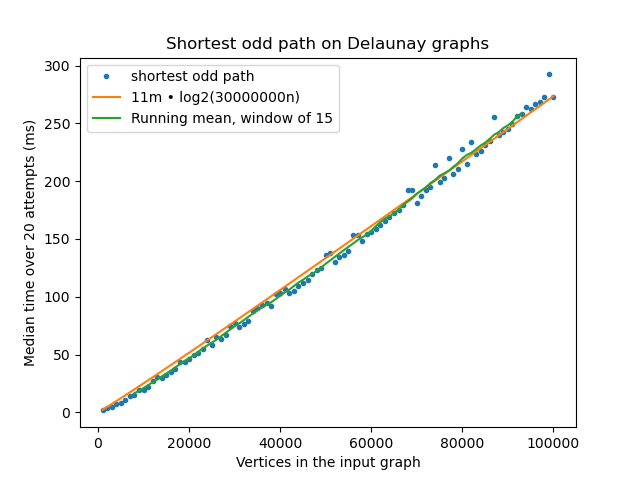
\includegraphics[width=15cm]{figures/bench_plots/shortest odd path.png}

As we can see, the running times grow almost linearly as the inputs grow larger. The slight upwards curve is barely noticable. This is to be expected with a linearithmic theoretical running time.

\subsection{Discussion}
The focus of this thesis is to create an algorithm that performs well on sparse graphs, especially planar graphs, which is why we consider the running times mainly on sparse graphs. If we instead had implemented an algorithm for denser graphs, or just graphs in general, then testing on graphs with more edges would be more appropriate.

With that said, we are very happy with these results. Being able to solve graphs of millions of nodes in seconds is exactly the performance we were hoping for.

\todo{write more here}

\chapter{Network Diversion}
\section{Intuition}
\subsection{Detour paths}
\label{section:subdividing-detours}
Before we reveal the algorithm for Network Diversion, we will first look at a curious little problem that we call \textsc{Shortest Detour Path}. Instead of deleting edges to force all paths to go through a certain edge, we want to purposefully pass through that edge and look for the shortest path that does. Perhaps we are going on a road trip, and we want to stop at a specific gas station along the road to say hi to our friend Mike who works there. And because this is a road trip, we do not want to drive along the same roads multiple times, that would be boring.

\problem
{Shortest Detour Path}
{a graph $G$, two vertices $s,t \in V$, and a 'detour' edge $d \in E$}
{an $s$-$t$-path in $G$ of minimum cost, that goes through the detour $d$}

There is no obvious way to solve \textsc{Shortest Detour Path}. One might attempt to concatenate the shortest $s$-$\from(d)$-path and the shortest $\too(d)$-$t$-path, but those two paths might overlap and reuse the same vertices, and therefore would their concatenation not necessarily be a path but instead a mere walk. The classical solution is to use a maximum flow algorithm like Edmonds-Karp \cite{source:edmonds-karp-algorithn} to find those two paths, to enforce that they are vertex-disjoint. It works, but is slower and more complicated compared to what we are about to do.

Instead, we create a new graph $H$, by subdividing all edges in $G$ \emph{except} $d$, as seen in \Cref{figure:subdividing-detours}. The key point to see here is that any odd $s$-$t$-path in $H$ must necessarily go through the detour, otherwise it would not be odd. We can visualize it by 'stepping through' the edges in $H$. If we start on our right leg, then in the beginning every time we reach a vertex that is also in $G$, we reach it by stepping on our left leg. That continues until we use the detour edge, and from then on we step on all vertices from $G$ using our right leg. If we require that we end at $t$ on our right leg, then the path must be odd, and any odd path must go through the detour. Therefore we can simply run our \textsc{Shortest Odd Path} algorithm on $H$, and if such a path exists we can reverse the subdivision of the edges in the path and the result is the \textsc{Shortest Detour Path} in $G$.

\begin{figure}[H]
    \centering
    \begin{subfigure}{.45\textwidth}
        \centering
        \scalebox{0.88}{
            \begin{tikzpicture}
                \tikzstyle{every node}=[circle, fill=lightgray, draw=black, inner sep=2pt, minimum size=1.5em, font=\footnotesize, text=black]
                \tikzstyle{edge}=[gray, line width=1.5mm]
            
                \node (s) at (0,0) {$s$};
                \node (a) at (1.5,1.5) {};
                \node (b) at (3,0) {};
                \node (c) at (1.5,-1.5) {};
                \node (d) at (4.5,-1.5) {};
                \node (e) at (6,0) {};
                \node (f) at (4.5,1.5) {};
                \node (t) at (7.5,1.5) {$t$};
            
                \draw[edge] (s) -- (a) -- (b) -- (e);
                \draw[edge] (c) -- (b) -- (d) -- (e) -- (f) -- (t);
                \draw[edge] (a) -- (f);
            
                \tikzstyle{edge}=[red, line width=1.5mm]
                \draw[edge] (c) -- (d);
            \end{tikzpicture}
        }
        \caption{An instance of \textsc{Shortest Deour Path}, the detour marked in red.}
        \label{figure:detour}
    \end{subfigure}\hfill%
    \begin{subfigure}{.45\textwidth}
        \centering
        \scalebox{0.88}{
            \begin{tikzpicture}
                \tikzstyle{every node}=[circle, fill=lightgray, draw=black, inner sep=2pt, minimum size=1.5em, font=\footnotesize, text=black]
                \tikzstyle{edge}=[gray, line width=1.5mm]
            
                \node (s) at (0,0) {$s$};
                \node (a) at (1.5,1.5) {};
                \node (b) at (3,0) {};
                \node (c) at (1.5,-1.5) {};
                \node (d) at (4.5,-1.5) {};
                \node (e) at (6,0) {};
                \node (f) at (4.5,1.5) {};
                \node (t) at (7.5,1.5) {$t$};
            
                \draw[edge] (s) -- (a) -- (b) -- (e);
                \draw[edge] (c) -- (b) -- (d) -- (e) -- (f) -- (t);
                \draw[edge] (a) -- (f);
            
                \tikzstyle{edge}=[red, line width=1.5mm]
                \draw[edge] (c) -- (d);

                \tikzstyle{every node}=[circle, fill=lightgray, draw=black, inner sep=2pt, minimum size=1em, font=\footnotesize, text=black]
                \node (sa) at (0.75,0.75) {};
                \node (af) at (3,1.5) {};
                \node (ab) at (2.25,0.75) {};
                \node (bc) at (2.25,-0.75) {};
                \node (bd) at (3.75,-0.75) {};
                \node (be) at (4.5,0) {};
                \node (de) at (5.25,-0.75) {};
                \node (ef) at (5.25,0.75) {};
                \node (ft) at (6,1.5) {};
            \end{tikzpicture}
        }
        \caption{All edges except the detour have been subdivided, to create an instance of \textsc{Shortest Odd Path}.}
        \label{figure:subdivided-detour}
    \end{subfigure}%
    \caption{\textsc{Shortest Detour Path} reduced to \textsc{Shortest Odd Path} by subdividing all edges except the detour.}
    \label{figure:subdividing-detours}
\end{figure}

If we extend the problem to have multiple detour edges, where we have to go through all of them in any order, then our idea will not work\footnote{This is a good thing, because otherwise we would have solved the \textsc{Traveling Salesman Problem} in polynomial time and complexity theory as we know it would break down.}.
The problem is that we have no way of knowing whether we have used the marked edges 1, 3, or 5, etc. times, because in all of them we hit vertices from $G$ using our right leg. We can, however, use this idea to find paths that use a certain set of edges an odd amount of times. As it turns out, that is exactly what we need to solve \textsc{Network Diversion}.

\subsection{From a dual path to a real diversion}
Remember, we want to find a minimum minimal $s$-$t$-cut in $G$ that includes the diversion edge~$d$.

Instead of looking for a minimal cut in $G$, let us look for a simple cycle in the dual graph $G^\star$, as is explained to be equivalent in \Cref{fact:dual-cycle-is-real-cut}. We can do this by finding a path in $G^\star$ that goes from and to the left and right faces of $d$, without using $d^\star$ itself, and then adding $d^\star$ at the end to complete the cycle. If the path found is also the shortest such path, then it corresponds to the \emph{minimum} minimal cut in $G$ that uses $d$, though it is not necessarily an $s$-$t$-cut.

To force $s$ and $t$ to end up in different components after the cut, we need some additional details. First, we find any $s$-$t$-path in $G$, not necessarily the shortest path. Then we subdivide all the edges in the dual graph \emph{except} those who cross edges on the found $s$-$t$-path. Now we can look for the shortest \emph{odd} path that goes from and to the left and right faces of $d$ in the subdivided dual graph, and add $d^\star$ at the end to make it a cycle. Like before, this corresponds to a minimum minimal cut in $G$ that uses $d$, but now it must also cross the edges in the found $s$-$t$-path an odd number of times, as explained in \Cref{section:subdividing-detours}. 

This cycle, and the found $s$-$t$-path, can be interpreted as curves in our embedding. The cycle can additionally be interpreted as a Jordan curve, and by the Jordan Curve Theorem, the cycle divides the plane into an 'inside' and an 'outside'. Since the curve of the $s$-$t$-path crosses the curve of the cycle an odd number of times, exactly one of its endpoints must be on the inside, as illustrated in \Cref{figure:jordan-curve-cuts}. The endpoints are $s$ and $t$, meaning that $s$ and $t$ end up in different components after the cut. It follows that this cut is an $s$-$t$-cut in $G$, specifically a minimum minimal $s$-$t$-cut in $G$ that uses $d$.

This is the main idea for our algorithm. It should be noted that we did not come up with this idea ourselves, but have to thank Pål Grønås Drange \cite{source:pål} for his as for now unpublished work on the subject.

\begin{figure}[H]
    \centering
    \begin{subfigure}{.30\textwidth}
        \centering
        \includesvg[width = 0.8\textwidth]{figures/jordan_curves/one_crossing.svg}
        \caption{The path crosses the cycle once, so exactly one of the endpoints is on the inside.}
    \end{subfigure}\hfill%
    \begin{subfigure}{.30\textwidth}
        \centering
        \includesvg[width = 0.8\textwidth]{figures/jordan_curves/two_crossings.svg}
        \caption{The path crosses the cycle twice, both endpoints are on the outside.}
    \end{subfigure}\hfill%
    \begin{subfigure}{.30\textwidth}
        \centering
        \includesvg[width = 0.8\textwidth]{figures/jordan_curves/three_crossings.svg}
        \caption{The path crosses the cycle thrice, so the endpoints must end up on either side of the cycle.}
    \end{subfigure}
    \caption{The two endpoints of a path end up on different sides of a cycle if and only if it crosses the cycle an odd number of times.}
    \label{figure:jordan-curve-cuts}
\end{figure}

\subsection{The algorithm}
\label{subsection:network-diversion-example}
We will explain the algorithm by following an example. We want to find the minimum minimal $s$-$t$-cut that includes the diversion edge marked in red. 

\begin{center}
\begin{tikzpicture}
    \tikzstyle{every node}=[circle, fill=lightgray, draw=black, inner sep=2pt, minimum size=1.5em, font=\footnotesize, text=black]
    \tikzstyle{edge}=[gray, line width=1mm]

    \node (s) at (0,0) {$s$};
    \node (a) at (2,-0.5) {};
    \node (b) at (1,-2) {};
    \node (c) at (1,1) {};
    \node (d) at (3.5,-1.5) {};
    \node (e) at (3,1) {};
    \node (f) at (-2,-1) {};
    \node (t) at (5,0) {$t$};
    \node (g) at (-1,-2.5) {};
    \node (h) at (3,2.5) {};
    \node (i) at (-0.75,2.5) {};
    \node (j) at (5,2) {};
    \node (k) at (-2.5,1.5) {};

    \draw[edge] (t) -- (j) -- (h) -- (i) -- (k) -- (f) -- (g) -- (b) -- (d) -- (e) -- (h);
    \draw[edge] (s) -- (c) -- (i) -- (f) -- (s);
    \draw[edge] (f) -- (b) -- (a) -- (d) -- (t);
    \draw[edge] (s) -- (a) -- (e) -> (t);

    \tikzstyle{edge}=[red, line width=1mm]
    \draw[edge] (c) -- (e);
\end{tikzpicture}
\end{center}

First, we find any $s$-$t$-path that does not use the diversion edge. It does not necessarily have to be the shortest path. We have marked such a path in green below.

\begin{center}
\begin{tikzpicture}
    \tikzstyle{every node}=[circle, fill=lightgray, draw=black, inner sep=2pt, minimum size=1.5em, font=\footnotesize, text=black]
    \tikzstyle{edge}=[gray, line width=1mm]

    \node (s) at (0,0) {$s$};
    \node (a) at (2,-0.5) {};
    \node (b) at (1,-2) {};
    \node (c) at (1,1) {};
    \node (d) at (3.5,-1.5) {};
    \node (e) at (3,1) {};
    \node (f) at (-2,-1) {};
    \node (t) at (5,0) {$t$};
    \node (g) at (-1,-2.5) {};
    \node (h) at (3,2.5) {};
    \node (i) at (-0.75,2.5) {};
    \node (j) at (5,2) {};
    \node (k) at (-2.5,1.5) {};

    \draw[edge] (t) -- (j) -- (h) -- (i) -- (k) -- (f) -- (g) -- (b) -- (d) -- (e) -- (h);
    \draw[edge] (s) -- (c) -- (i) -- (f) -- (s);
    \draw[edge] (f) -- (b) -- (a) -- (d) -- (t);

    \tikzstyle{edge}=[red, line width=1mm]
    \draw[edge] (c) -- (e);

    \tikzstyle{edge}=[green, line width=1mm]
    \draw[edge] (s) -- (a) -- (e) -> (t);
\end{tikzpicture}
\end{center}

Next up is to compute the dual graph. We delete the dual edge that crosses the diversion edge and color the rest in blue. Note that we have omitted the outside face and its edges in this visualization, otherwise we would have a much too cluttered illustration.

\begin{center}
\begin{tikzpicture}
    \tikzstyle{every node}=[circle, fill=lightgray, draw=black, inner sep=2pt, minimum size=1.5em, font=\footnotesize, text=black]
    \tikzstyle{edge}=[gray, line width=1mm]

    \node (s) at (0,0) {$s$};
    \node (a) at (2,-0.5) {};
    \node (b) at (1,-2) {};
    \node (c) at (1,1) {};
    \node (d) at (3.5,-1.5) {};
    \node (e) at (3,1) {};
    \node (f) at (-2,-1) {};
    \node (t) at (5,0) {$t$};
    \node (g) at (-1,-2.5) {};
    \node (h) at (3,2.5) {};
    \node (i) at (-0.75,2.5) {};
    \node (j) at (5,2) {};
    \node (k) at (-2.5,1.5) {};

    \draw[edge] (t) -- (j) -- (h) -- (i) -- (k) -- (f) -- (g) -- (b) -- (d) -- (e) -- (h);
    \draw[edge] (s) -- (c) -- (i) -- (f) -- (s);
    \draw[edge] (f) -- (b) -- (a) -- (d) -- (t);

    \tikzstyle{edge}=[red, line width=1mm]
    \draw[edge] (c) -- (e);

    \tikzstyle{edge}=[green, line width=1mm]
    \draw[edge] (s) -- (a) -- (e) -> (t);

    \tikzstyle{every node}=[circle, draw=blue, fill=cyan, inner sep=2pt, minimum size=0.7em]
    \node (aces) at (1.5,0.5) {};
    \node (cehi) at (2,1.75) {};
    \node (ehjt) at (4,1.25) {};
    \node (det) at (4,-0.25) {};
    \node (ade) at (2.75,-0.3) {};
    \node (abd) at (2,-1.25) {};
    \node (abfs) at (0,-1) {};
    \node (bfg) at (-0.75,-1.75) {};
    \node (cifs) at (-0.75,1) {};
    \node (fik) at (-1.75,1.25) {};

    \tikzstyle{edge}=[blue, line width=0.7mm]
    \draw[edge] (fik) -- (cifs) -- (cehi) -- (ehjt) -- (det) -- (ade) -- (abd) -- (abfs) -- (bfg);
    \draw[edge] (ade) -- (aces) to [bend left=20] (cifs) to [bend right=25] (abfs) to [bend right=20] (aces); 
\end{tikzpicture}
\end{center}

Now we subdivide all the edges in the dual graph except those that cross the path in green.

\begin{center}
\begin{tikzpicture}
    \tikzstyle{every node}=[circle, fill=lightgray, draw=black, inner sep=2pt, minimum size=1.5em, font=\footnotesize, text=black]
    \tikzstyle{edge}=[gray, line width=1mm]

    \node (s) at (0,0) {$s$};
    \node (a) at (2,-0.5) {};
    \node (b) at (1,-2) {};
    \node (c) at (1,1) {};
    \node (d) at (3.5,-1.5) {};
    \node (e) at (3,1) {};
    \node (f) at (-2,-1) {};
    \node (t) at (5,0) {$t$};
    \node (g) at (-1,-2.5) {};
    \node (h) at (3,2.5) {};
    \node (i) at (-0.75,2.5) {};
    \node (j) at (5,2) {};
    \node (k) at (-2.5,1.5) {};

    \draw[edge] (t) -- (j) -- (h) -- (i) -- (k) -- (f) -- (g) -- (b) -- (d) -- (e) -- (h);
    \draw[edge] (s) -- (c) -- (i) -- (f) -- (s);
    \draw[edge] (f) -- (b) -- (a) -- (d) -- (t);

    \tikzstyle{edge}=[red, line width=1mm]
    \draw[edge] (c) -- (e);

    \tikzstyle{edge}=[green, line width=1mm]
    \draw[edge] (s) -- (a) -- (e) -> (t);

    \tikzstyle{every node}=[circle, draw=blue, fill=cyan, inner sep=2pt, minimum size=0.75em]
    \node (aces) at (1.5,0.5) {};
    \node (cehi) at (2,1.75) {};
    \node (ehjt) at (4,1.25) {};
    \node (det) at (4,-0.25) {};
    \node (ade) at (2.75,-0.3) {};
    \node (abd) at (2,-1.25) {};
    \node (abfs) at (0,-1) {};
    \node (bfg) at (-0.75,-1.75) {};
    \node (cifs) at (-0.75,1) {};
    \node (fik) at (-1.75,1.25) {};


    \tikzstyle{every node}=[circle, draw=blue, fill=cyan, inner sep=2pt, minimum size=0.35em]
    \node (fi) at (-1.4,1) {};
    \node (fs) at (-0.75,-0.5) {};
    \node (bf) at (-0.35,-1.5) {};
    \node (ci) at (0.5,1.75) {};
    \node (eh) at (3,1.75) {};
    \node (de) at (3.25,-0.5) {};
    \node (ad) at (2.5,-1) {};
    \node (ab) at (1.5,-1.25) {};

    \tikzstyle{edge}=[blue, line width=0.7mm]
    \draw[edge] (fik) -- (fi) -- (cifs) -- (ci) -- (cehi) -- (eh) -- (ehjt) -- (det) -- (de) -- (ade) -- (ad) -- (abd) -- (ab) -- (abfs) -- (bf) -- (bfg);
    \draw[edge] (ade) -- (aces) to [bend left=20] (cifs) -- (fs) -- (abfs) to [bend right=20] (aces);    
\end{tikzpicture}
\end{center}

The last step is to find the shortest odd path in the subdivided dual graph from and to the regions to the left and right of the diversion edge, using our newfound favorite algorithm. If we find such a path, we know that it must cross the $s$-$t$-path in green an odd number of times. If we add the dual equivalent of the diversion edge to the path to create a cycle, then we know that this cycle goes around either $s$ or $t$, but not both. We illustrate the cycle in orange below.

\begin{center}
\begin{tikzpicture}
    \tikzstyle{every node}=[circle, fill=lightgray, draw=black, inner sep=2pt, minimum size=1.5em, font=\footnotesize, text=black]
    \tikzstyle{edge}=[gray, line width=1mm]

    \node (s) at (0,0) {$s$};
    \node (a) at (2,-0.5) {};
    \node (b) at (1,-2) {};
    \node (c) at (1,1) {};
    \node (d) at (3.5,-1.5) {};
    \node (e) at (3,1) {};
    \node (f) at (-2,-1) {};
    \node (t) at (5,0) {$t$};
    \node (g) at (-1,-2.5) {};
    \node (h) at (3,2.5) {};
    \node (i) at (-0.75,2.5) {};
    \node (j) at (5,2) {};
    \node (k) at (-2.5,1.5) {};

    \draw[edge] (t) -- (j) -- (h) -- (i) -- (k) -- (f) -- (g) -- (b) -- (d) -- (e) -- (h);
    \draw[edge] (s) -- (c) -- (i) -- (f) -- (s);
    \draw[edge] (f) -- (b) -- (a) -- (d) -- (t);

    \tikzstyle{edge}=[red, line width=1mm]
    \draw[edge] (c) -- (e);

    \tikzstyle{edge}=[green, line width=1mm]
    \draw[edge] (s) -- (a) -- (e) -> (t);

    \tikzstyle{every node}=[circle, draw=blue, fill=cyan, inner sep=2pt, minimum size=0.75em]
    \node (aces) at (1.5,0.5) {};
    \node (cehi) at (2,1.75) {};
    \node (ehjt) at (4,1.25) {};
    \node (det) at (4,-0.25) {};
    \node (ade) at (2.75,-0.3) {};
    \node (abd) at (2,-1.25) {};
    \node (abfs) at (0,-1) {};
    \node (bfg) at (-0.75,-1.75) {};
    \node (cifs) at (-0.75,1) {};
    \node (fik) at (-1.75,1.25) {};


    \tikzstyle{every node}=[circle, draw=blue, fill=cyan, inner sep=2pt, minimum size=0.35em]
    \node (fi) at (-1.4,1) {};
    \node (fs) at (-0.75,-0.5) {};
    \node (bf) at (-0.35,-1.5) {};
    \node (ci) at (0.5,1.75) {};
    \node (eh) at (3,1.75) {};
    \node (de) at (3.25,-0.5) {};
    \node (ad) at (2.5,-1) {};
    \node (ab) at (1.5,-1.25) {};

    \tikzstyle{edge}=[blue, line width=0.7mm]
    \draw[edge] (fik) -- (fi) -- (cifs);
    \draw[edge] (cehi) -- (eh) -- (ehjt) -- (det) -- (de) -- (ade) -- (ad) -- (abd) -- (ab) -- (abfs) -- (bf) -- (bfg);
    \draw[edge] (ade) -- (aces) to [bend left=20] (cifs);

    \tikzstyle{edge}=[orange, line width=0.9mm]
    \draw[edge] (cehi) -- (ci) -- (cifs) -- (fs) -- (abfs) to [bend right=20] (aces);
    \draw[edge] (aces) -- (cehi);
\end{tikzpicture}
\end{center}

With this, we finally have our diversion set. Simply delete the edges in the original graph that cross the cycle in orange, except for the diversion edge of course. We end up with a graph where all $s$-$t$-paths must pass through the diversion edge. The problem is solved.

\begin{center}
\begin{tikzpicture}
    \tikzstyle{every node}=[circle, fill=lightgray, draw=black, inner sep=2pt, minimum size=1.5em, font=\footnotesize, text=black]
    \tikzstyle{edge}=[gray, line width=1mm]

    \node (s) at (0,0) {$s$};
    \node (a) at (2,-0.5) {};
    \node (b) at (1,-2) {};
    \node (c) at (1,1) {};
    \node (d) at (3.5,-1.5) {};
    \node (e) at (3,1) {};
    \node (f) at (-2,-1) {};
    \node (t) at (5,0) {$t$};
    \node (g) at (-1,-2.5) {};
    \node (h) at (3,2.5) {};
    \node (i) at (-0.75,2.5) {};
    \node (j) at (5,2) {};
    \node (k) at (-2.5,1.5) {};

    \draw[edge] (t) -- (j) -- (h) -- (i) -- (k) -- (f) -- (g) -- (b) -- (d) -- (e) -- (h);
    \draw[edge] (c) -- (s);
    \draw[edge] (a) -- (e) -- (t);
    \draw[edge] (i) -- (f) -- (b) -- (a) -- (d) -- (t);

    \tikzstyle{edge}=[red, line width=1mm]
    \draw[edge] (c) -- (e);
\end{tikzpicture}
\end{center}
\section{Psuedocode}
\begin{lstlisting}[caption={Main},label=Listing,mathescape=true]
network_diversion(PlanarGraph graph, s, t, Edge diversion) -> Option<(int, List<Edge>)> {
    let `path` be any s-t-path that does not use the diversion edge;
}
\end{lstlisting}
\section{Analysis}

\begin{theorem}
    Let $(G, s, t, d)$ be an instance of \textsc{Network Diversion}, and let $n~:= |V|$. \\
    Claim: our algorithm runs in time $O(n \log n)$.
    
    \begin{proof}
        We find first a shortest $s$-$t$-path in $G$ that does not use $d$, in time $O(n+m)$.
    
        Then we subdivide all the edges in $G^\star$ except those found in the path, in time $O(n+m)$. This new graph has size $n' \leq 2n \in O(n)$ and $m' \leq 2m \in O(m)$.
    
        Next up is to find an odd path in the subdivided graph, in time $O(m' \log n') = O(m \log n)$.
    
        Lastly, if we are interested in the specific set of edges in the diversion and not just the cost, we un-subdivide the odd path in time $O(n') = O(n)$.
    
        In total, we have a running time of $O(n+m) + O(m \log n) + O(n) = O(m \log n)$. Since $G$ is planar we have that $m \in O(n)$, so we can simplify the complexity to just $O(n \log n)$ and complete the proof.
    \end{proof}
\end{theorem}

Note that here we have assumed that the dual graph $G^\star$ has already been computed prior to starting the algorithm. If we have a straight-line embedding of $G$ we can compute $G^\star$ in $O(n+m)$, which would not change the overall running time. However, if we do not have such an embedding the total running time might be considerably more.

We compare the theoretical and practical running times on Delaunay graphs as we did in \Cref{subsubsection:odd-path-delaunay-testing}. For each graph, we have estimated a source and target vertex of maximum distance between each other and picked three edges in the graph as diversion edges. We select whichever diversion edge leads to the worst meadian running time over 10 runs, and plot the results below.

Here too have we tried to create a function out of the theoretical running time of $O(n \log n)$, this time with different constants. We have set $m~:= 3n$ in the plot since the graphs are planar.

\begin{center}
    \includesvg[width=0.9\textwidth]{figures/bench_plots/network diversion.svg}    
\end{center}

As we can see, the running times grow just barely more than linearly compared to the input size. This is not surprising considering the linearithmic theoretical running time. The algorithm easily solves \textsc{Network Diversion} on planar graphs of 100000 vertices in less than a second. Now compare that to the existing algorithms that will need more than a second to solve for more than 30 vertices, and it is clear why a polynomial running time matters so much.

See \Cref{figure:network-diversion-on-delaunay} for yet another example of what a diversion set may look like, this time on a Delaunay graph of 35 vertices.

\noindent
\begin{figure}
    \centering
    \begin{subfigure}{.32\textwidth}
        \centering
        \includesvg[width=\textwidth]{figures/diversions/delaunay35-Full.svg}
        \caption{$s$ and $t$ are marked in blue, the diversion edge in red}
        \label{subfigure:network-diversion-input}
    \end{subfigure}\hfill%
    \begin{subfigure}{.32\textwidth}
        \centering
        \includesvg[width=\textwidth]{figures/diversions/delaunay35-Partial.svg}
        \caption{One possible diversion set marked in orange}
        \label{subfigure:network-diversion-diversion}
    \end{subfigure}\hfill%
    \begin{subfigure}{.32\textwidth}
        \centering
        \includesvg[width=\textwidth]{figures/diversions/delaunay35-Diverted.svg}
        \caption{With the diversion set removed, all $s$-$t$-paths must go through the diversion edge}
        \label{subfigure:network-diversion-diverted}
    \end{subfigure}
    \caption{Example of a solution for \textsc{Network Diversion} on a Delaunay graph of 35 vertices}
    \label{figure:network-diversion-on-delaunay}
\end{figure}


\chapter{Conclusion}

\todo[inline]{Should really write some sort of conclusion or something one of these days}

% Include more chapters as required.
%%=========================================

% Alternative 1 of printing glossaries & acronymes
%\renewcommand{\glossarypreamble}{\footnotesize}
%\printglossary[style=super, type=\glsdefaulttype] \let\cleardoublepage\clearpage
%\printglossary[style=super, type=\acronymtype]


%Alternative 2
%Simplified way of printing glossaries, slower than alt 1, but has better compatibility
\printnoidxglossaries

% Include more appendices as required.
%%=========================================
\clearpage
\DeclareRobustCommand{\VAN}[3]{#3}
\addcontentsline{toc}{chapter}{Bibliography}

\bibliography{generators/refs.bib}
\bibliographystyle{alpha}

\appendix
\titleformat{\chapter}[display]
  {\normalfont\large\bfseries}% <- font for label "Appendix A", default \huge
  {\chaptertitlename\ \thechapter}
  {20pt}
  {\large}% <- font for title, default \Huge

% \chapter{Generated code from Protocol buffers}

\begin{lstlisting}[caption={Source code of something},label=Listing]
System.out.println("Hello Mars");
\end{lstlisting}
\end{document}
